% -------------------------------------------------------------------------------------------------
%      MDSG Latex Framework
%      ============================================================================================
%      File:                  main.tex
%      Author(s):             Michael Duerr
%      Version:               1
%      Creation Date:         30. Mai 2010
%      Creation Date:         30. Mai 2010
%
%      Notes:                 - This represents the document root of this template
%                             - Binding correction is 12mm. In case you change this value, you
%                               may also need to adapt the value of \bcorlength in mdsg.sty
%                             - Switch `babel' package options `english' and `ngerman' in case
%                               your thesis is in English
%                             - if you prefer to use utf8 encoding, uncomment the corresponding
%                               line `\usepackage[utf8]{inputenc}' and comment the line
%                               `\usepackage[latin1]{inputenc}'. To compile this example you also
%                               need to include the corresponding introduction example file i.e.
%                               `introduction-UTF8.tex' or `introduction-ISO8859-1.tex'
% -------------------------------------------------------------------------------------------------
%
\documentclass[enabledeprecatedfontcommands,bibliography=totoc,listof=totoc,index=totoc,twoside=true,BCOR=12mm,DIV=12]{scrbook}
%\KOMAoptions{draft=true}                         % uncomment if you want to visualise overful hbox
%\KOMAoptions{chapterprefix=true}                 % uncomment if you like "Chapter" in front of
                                                  % chapter number
%\KOMAoptions{appendixprefix=true}                % uncomment if you like "Appendix" in front of
                                                  % appendix number
%\KOMAoptions{...}                                % feel free to add additional KOMA options
%
% =================================================================================================
% set encoding
% -------------------------------------------------------------------------------------------------
%
\usepackage[utf8]{inputenc}                       % uncomment if you prefer utf8 encoding
%\usepackage[latin1]{inputenc}                    % uncomment if you prefer latin1 encoding
%
% =================================================================================================
% load mdsg style
% -------------------------------------------------------------------------------------------------
%
%\usepackage[diplom]{mdsg}                        % uncomment the corresponding option
%\usepackage[fopra]{mdsg}
\usepackage[bachelor]{mdsg}
%\usepackage[master]{mdsg}
%
% =================================================================================================
% initialize macros
% -------------------------------------------------------------------------------------------------
%
\lmutitle{Basket Option Pricing with Quantum Circuits}                       % title: you can force a new line by
%\lmutitle{Titel \\ der \\ Arbeit}                % inserting `\\'. However, this will cause
                                                  % a hyperref warning!
\lmustudentone{Moritz Maier}                    % first author's name
%\lmustudenttwo{Max2 Mustermann2}                 % second author's name
%\lmustudentthree{Max3 Mustermann3}               % third author's name
%\lmustudentfour{Max4 Mustermann4}                % fourth author's name

\lmuprofone{Prof. Dr. Claudia Linnhoff-Popien}    % first supervisor's name
% \lmuproftwo{Prof. Dr. Max Mustermann}             % second supervisor's name
                                                  % (uncomment if not needed)
% \lmuprofthree{Prof. Dr. Max2 Mustermann2}         % third supervisor's name
                                                  % (uncomment if not needed)
\lmuadvisorone{Michael Poppel}                    % first advisor's name
\lmuadvisortwo{Tobias Rohe}                    % second advisor's name
                                                  % (uncomment if not needed)
% \lmuadvisorthree{Betreuer Name3}                  % third advisor's name
                                                  % (uncomment if not needed)
\lmudraftdate{\today}                             % only for versioning during work!
                                                  % (uncomment for final version!)
\lmudeadline{9. März 2026}                      % deadline (day of submission)
%
% =================================================================================================
% package selection (add additional packages if needed)
% -------------------------------------------------------------------------------------------------
%
%\usepackage{layout}                              % see documentation of this package
\usepackage{cmap}                                 % to produce searchable PDF
\usepackage[T1]{fontenc}                          % split german words with umlaut
\usepackage{lmodern}
\usepackage[ngerman, english]{babel}               % for german toc, ...
% \usepackage{bibgerm}                              % for german bibliography index
\usepackage{tabularx}                             % more flexible table environment
\usepackage{booktabs}                             % high quality tables
\usepackage{rotating}                             % for generation of landscape tables
\usepackage{multirow}                             % for multirow cells inside tables
\usepackage{amssymb,amsmath}                      % powerful math package
\usepackage{hyperref}    
% \usepackage[hidelinks]{hyperref}% for hyperlinks
\lmuhypersetup                                    % write some pdf properties
\usepackage{flafter}                              % force floats to appear after their reference
\usepackage{subfig}                               % to allow for side by side graphics (subfloats)
\usepackage{pdflscape}                            % enable rotation of landscape pages
\usepackage{hyphenat}                             % proper hyphenation for bla_bla to bla_-bla
\usepackage[all]{hypcap}                          % correct captions
\usepackage{url}                                  % nicer url style
\usepackage{enumitem}                             % for tight lists
% \usepackage{quantikz}    
\usepackage{tikz}
\usepackage{quantikz}

\setcounter{tocdepth}{3}                          % sectioning depth in toc
\setcounter{secnumdepth}{3}                       % sectioning depth in text

\graphicspath{{./pictures/}}                      % put all graphics here
\input{hyphenation}                               % this file holds words latex cannot split
%
% =================================================================================================
% start of document
% -------------------------------------------------------------------------------------------------
%

\usepackage{verbatim}
\begin{document}
    \setlist{noitemsep}                           % for tight lists
    \lmufront                                     % title pages
    \newpage
    \cleardoublepage
    \lmuaffirmation                               % affirmation (work is my own work)
    \newpage
    \cleardoubleemptypage
    \thispagestyle{empty}
    % -------------------------------------------------------------------------------------------------
%      MDSG Latex Framework
%      ============================================================================================
%      File:                  abstract.tex
%      Author(s):             Michael Duerr
%      Version:               1
%      Creation Date:         30. Mai 2010
%      Creation Date:         30. Mai 2010
%
%      Notes:                 - Place your abstract here
% -------------------------------------------------------------------------------------------------
%
\vspace*{2cm}

\begin{center}
    \textbf{Abstract}
\end{center}

\vspace*{1cm}

\noindent Die Bewertung von Basket-Optionen stellt aufgrund der Abhängigkeit von mehreren Underlyings und deren Korrelationen eine komplexe numerische Herausforderung dar. Während klassische Monte-Carlo-Verfahren mit zunehmender Dimension hohen Rechenaufwand erfordern, ermöglichen Machine-Learning-Ansätze eine direkte Approximation der Preisfunktion. Ziel dieser Arbeit ist die Untersuchung variationaler Quantenschaltkreise (VQCs) zur Approximation von Basket-Optionspreisen sowie der Vergleich mit etablierten klassischen neuronalen Netzarchitekturen. Die Trainingsdaten basieren auf Monte-Carlo-Simulationen, deren Parameter aus historischen Marktdaten geschätzt werden. Es werden unterschiedliche Payoff-Strukturen (Worst-of, Best-of, Average) betrachtet sowie die Einflüsse von Trainingsdatensatzgröße, künstlichem Rauschen und einem zeitlich geordneten Train-Test-Split analysiert. Zusätzlich wird die Frequenzstruktur der Zielgrößen mithilfe einer Non-Uniform Fast Fourier Transform untersucht, um die darstellbare Modellkapazität der VQCs spektral einzuordnen. Die Ergebnisse zeigen, dass sowohl klassische neuronale Netze als auch VQC-basierte Modelle die Preisfunktion mit hoher Genauigkeit approximieren können. Während klassische Netze tendenziell von zunehmender Modellgröße profitieren, erreichen VQCs bereits bei moderater Schaltkreistiefe einen Großteil ihrer maximalen Leistungsfähigkeit, was mit der überwiegend niederfrequenten Struktur der Zielgrößen konsistent ist. Unter begrenzter Datenverfügbarkeit und starkem Rauschen erweisen sich einfachere Modelle als robuster, während komplexere Architekturen erst bei ausreichender Datenmenge ihr Potenzial entfalten. Insgesamt erreichen VQC-basierte Modelle eine konkurrenzfähige Approximationsleistung, ohne jedoch einen klaren Vorteil gegenüber klassischen neuronalen Netzen zu zeigen.                       % abstract
	\newpage
    \cleardoubleemptypage
    \thispagestyle{empty}
	% -------------------------------------------------------------------------------------------------
%      MDSG Latex Framework
%      ============================================================================================
%      File:                  abstract.tex
%      Author(s):             Michael Duerr
%      Version:               1
%      Creation Date:         30. Mai 2010
%      Creation Date:         30. Mai 2010
%
%      Notes:                 - Place your abstract here
% -------------------------------------------------------------------------------------------------
%
\vspace*{2cm}

\begin{center}
    \textbf{Abstract}
\end{center}

\vspace*{1cm}

\noindent The valuation of basket options poses a complex numerical challenge due to their dependence on multiple underlying assets and their correlations. While classical Monte Carlo methods require substantial computational effort as the dimensionality increases, machine learning approaches enable a direct approximation of the pricing function. The objective of this thesis is to investigate variational quantum circuits (VQCs) for approximating basket option prices and to compare their performance with established classical neural network architectures. The training data are generated using Monte Carlo simulations whose parameters are estimated from historical market data. Different payoff structures (Worst-of, Best-of, and Average) are considered, and the effects of training dataset size, artificial noise, and a temporally ordered train–test split are analyzed. In addition, the frequency structure of the target functions is examined using a Non-Uniform Fast Fourier Transform in order to relate the representational capacity of the VQCs to the spectral properties of the pricing function. The results show that both classical neural networks and VQC-based models can approximate the pricing function with high accuracy. While classical networks tend to benefit from increasing model size, VQCs achieve most of their maximum performance already at moderate circuit depth, which is consistent with the predominantly low-frequency structure of the target functions. Under limited data availability and strong noise, simpler models prove to be more robust, whereas more complex architectures only reach their full potential when sufficient training data are available. Overall, VQC-based models achieve a competitive approximation performance, although they do not demonstrate a clear advantage over classical neural networks in the investigated setting.
    \thispagestyle{empty}
    \frontmatter                                  % start roman numbering
    \tableofcontents                              % toc
    \mainmatter                                   % start alpha numbering
%
% =================================================================================================
% place your document text here (take care of encoding)
% -------------------------------------------------------------------------------------------------
%
    \chapter{Introduction}

The valuation of options is one of the central problems in quantitative financial mathematics. While closed-form solutions exist for simple European options -- most notably within the Black--Scholes framework -- the pricing of more complex derivatives is considerably more challenging. In particular, so-called basket options, whose payoff depends on multiple underlyings, generally require numerical methods such as Monte Carlo simulations. As the number of underlying assets increases, the computational effort grows substantially, since correlations between the assets must also be taken into account.

In recent years, machine learning methods have emerged as a powerful alternative to classical analytical and numerical valuation techniques. Instead of explicitly specifying a stochastic model for the dynamics of the underlyings, neural networks learn the functional relationship between input variables and the option price directly. After the training phase, the valuation of new configurations can be performed with low computational cost. Studies such as \cite{culkin2017machine} and \cite{ferguson2018deeply} demonstrate that deep neural networks are capable of approximating even complex basket option prices with high accuracy.

Parallel to these developments, quantum computing has emerged as a promising field of research. Variational quantum circuits (VQCs) represent a hybrid approach in which a parameterized quantum circuit is trained using classical optimization procedures. Due to their structurally different functional representation, VQCs differ fundamentally from classical neural networks. While classical models realize nonlinearity through explicit activation functions and typically produce piecewise linear approximations, nonlinear dependencies in a VQC arise implicitly from the parameterized unitary transformation and the subsequent measurement process.

In the context of basket options, the question arises whether the inherent ability of entangled quantum states to represent non-separable dependencies can provide advantages in modeling correlated financial quantities. Since the payoff of a basket option depends crucially on the joint distribution of multiple underlyings, it is natural to investigate to what extent the global interactions between qubits enabled by entanglement can contribute to capturing such dependency structures.

The objective of this thesis is to investigate the approximation of basket option prices using a VQC. As freely available historical datasets of actually traded basket options are only very limited, data generation is based on a simulation model. Volatilities and correlations are estimated from real historical time series and used within a Monte Carlo simulation framework. The resulting prices therefore represent model-based target values. The datasets generated in this way serve as the training and test basis for the models under consideration.

The focus lies on the comparison between a quantum machine learning model in the form of a VQC and established classical neural network architectures following \cite{culkin2017machine} and \cite{ferguson2018deeply}. Different dataset sizes as well as various basket payoff structures (Worst-of, Best-of, Average) are considered, and the influence of noise is also examined.

The thesis is structured as follows:
First, the theoretical foundations of basket options, Monte Carlo simulation, classical neural networks, and VQCs are presented. Subsequently, the methodology for data generation, model architecture, and training procedure is described. Building upon this, the experimental results are presented and discussed with regard to the performance of the quantum- and classical-based models. Finally, the findings are summarized and possible directions for future research are outlined.
    \chapter{Background}
\label{sec:background}

\section{Options and Derivatives}
\label{sec:bg-options}

Financial derivatives are contracts whose value depends on the performance of one or more underlying assets. These can include, for example, stocks, bonds, indices, or commodities. Derivatives are used both for hedging risks and for speculating on price movements.

Options are a central class of derivatives that give the holder the right, but not the obligation, to buy (call) or sell (put) an underlying asset at a predetermined price (strike) at a fixed expiration date (European-style).

The payoff of a simple call option on an underlying asset $S_T$ with strike $K$ can be expressed mathematically as
\begin{equation}
\text{Payoff}_{\text{Call}} = \max(S_T - K, 0),
\end{equation}
where $S_T$ denotes the price of the underlying asset at maturity $T$. 
Since $S_T$ is a future and therefore uncertain quantity, its distribution must be modeled in order to determine the present value of the option.

\section{Basket Options}
\label{sec:bg-basket-options}

Basket options are financial derivatives whose payouts depend on the performance of multiple underlying assets. They are frequently used in portfolio management or risk management to diversify the risk of individual assets. Unlike simple options on a single underlying, a basket option considers multiple stocks, indices, or other assets simultaneously. The payoff depends on an aggregation of the individual underlying assets, for example:

\begin{itemize}
    \item \textbf{Worst-of option:} the payout is based on the asset with the worst performance.
    \item \textbf{Best-of option:} the payout is based on the asset with the best performance.
    \item \textbf{Average option:} the payout is based on the arithmetic mean of the returns or prices of the underlying assets.
\end{itemize}

Mathematically, the payoff of a basket option can generally be expressed as a function of the terminal prices of the included assets:
\begin{equation}
\text{Payoff} = f(S_T^{1}, S_T^{2}, \dots, S_T^{n}),
\end{equation}
where $S_T^{i}$ denotes the price of the $i$-th underlying asset at maturity $T$.

Specifically, for the three commonly used aggregation methods, the payoffs are given by:

\begin{align}
\text{Worst-of:} \quad & \text{Payoff}_{\text{worst}} = \max\!\left(\min_i S_T^{i} - K,\, 0\right),\\
\text{Best-of:} \quad & \text{Payoff}_{\text{best}} = \max\!\left(\max_i S_T^{i} - K,\, 0\right),\\
\text{Average:} \quad & \text{Payoff}_{\text{avg}} = \max\!\left(\frac{1}{n}\sum_{i=1}^{n} S_T^{i} - K,\, 0\right),
\end{align}

where $K$ is the strike price of the option.

Valuing basket options is more complex than single-asset options due to the dependencies among the underlying assets. These dependencies are typically modeled using the correlations between the individual assets. While closed-form solutions such as the Black-Scholes model \cite{black1973pricing} exist for simple options, they are only available under restrictive assumptions for basket options. Therefore, numerical methods, such as Monte Carlo simulation, are commonly employed.


\section{Monte Carlo Simulation for Basket Options}
\label{sec:bg-monte-carlo}
The Monte Carlo simulation \cite{boyle1977options} is a numerical method used to estimate the fair price of options by repeatedly simulating possible future paths of the underlying assets.

For each underlying asset $S_t^{i}$, the future price at time $T$ under
risk-neutral dynamics follows a geometric Brownian motion and is given by
\begin{equation}
S_T^{i}
=
S_0^{i}
\exp\!\left(
    (r - \tfrac{1}{2}\sigma_i^2) T
    +
    \sigma_i \sqrt{T}\, Z_i
\right),
\label{eq:bg-GBM}
\end{equation}
where $\sigma_i$ denotes the volatility of the $i$-th asset,
$r$ is the continuously compounded risk-free interest rate,
and $Z_i \sim \mathcal{N}(0,1)$ are standard normally distributed random variables.

Since basket options involve multiple underlying assets, the random variables $Z_i$ must reflect their empirically observed correlations. This is achieved via the Cholesky decomposition of the correlation matrix $\mathbf{C}$:
\begin{equation}
\mathbf{C} = \mathbf{L}\mathbf{L}^\top.
\label{eq:bg-Cholesky}
\end{equation}

Uncorrelated standard normal vectors $\mathbf{Z} \sim \mathcal{N}(0,I)$ are transformed into correlated random variables via
\begin{equation}
\mathbf{Z}_{\text{corr}} = \mathbf{L}\mathbf{Z}.
\end{equation}

The $i$-th component of the correlated vector is then used in \eqref{eq:bg-GBM},
\[
Z_i = \big(\mathbf Z_{\text{corr}}\big)_i .
\]

Under risk-neutral valuation, the option price is obtained as the discounted
expected value of the simulated payoffs:
\begin{equation}
\text{Price}
=
e^{-rT}
\cdot
\frac{1}{N}
\sum_{k=1}^{N}
\text{Payoff}_k.
\end{equation}

As the number of simulation paths $N$ increases, the estimator converges to the true expected value.

A practical limitation of Monte Carlo methods is their computational cost. 
The statistical error of the estimator decreases only on the order of
$\mathcal{O}(1/\sqrt{N})$, where $N$ is the number of simulated paths. 
Therefore, achieving higher accuracy requires a disproportionately large increase 
in simulation runs, which becomes particularly expensive for high-dimensional 
products such as basket options. 
Moreover, incorporating correlations between multiple underlying assets
requires an additional linear transformation of the simulated random variables,
leading to computational effort that grows approximately quadratically
with the number of assets.



    
\section{Machine Learning}
\label{sec:bg-machine-learning}

In contrast to classical rule-based algorithms, machine learning models learn functional relationships directly from observed data.

On classical computers, artificial neural networks (ANNs) are commonly used for this purpose. Their structure is inspired by biological nervous systems. These models consist of trainable parameters that are adjusted during an optimization process in order to minimize a target function.

In addition to classical neural networks, there also exist quantum-based machine learning approaches, such as VQCs. These consist of parameterized quantum gates whose parameters are optimized during training analogously to the weights of neural networks.

Such models are prone to overfitting, a phenomenon in which a model fits the training data too closely and consequently exhibits poorer performance on unseen data \cite{Goodfellow-et-al-2016}. To detect this effect, datasets are typically divided into training and test sets.

\subsection{Classical Neural Networks}
\label{sec:bg-classical-nn}

A neural network is organized into a sequence of layers, each containing at least one neuron. The first layer is referred to as the input layer and receives the original input data of the model. The last layer is the output layer and produces the model prediction. All layers between the input and output layer are called hidden layers.

A neural network in which data are propagated exclusively in one direction—from the input layer to the output layer—is referred to as a feedforward neural network.

Each neuron in a layer is typically connected to all neurons in the immediately following layer. Each neuron receives the outputs of the previous layer as input and forwards its own output to the next layer.

A neuron $h_n^{(j)}$ in the $n$-th layer of the neural network receives the outputs
$h_{n-1}^{(i)}$, $i = 1,2,\ldots,M_{n-1}$, of the previous layer as inputs. From these, the so-called net input is first computed:
\begin{equation}
a_n^{(j)} = \sum_{i=1}^{M_{n-1}} w_{ij}\, h_{n-1}^{(i)} + b_n^{(j)},
\end{equation}
where $M_{n-1}$ denotes the number of neurons in layer $(n-1)$. The weights $w_{ij}$ describe the strength of the connection between the $i$-th neuron of the previous layer and the $j$-th neuron of the current layer. The term $b_n^{(j)}$ represents the bias of the neuron.

The model parameters to be determined between layers $(n-1)$ and $n$ are thus given by
\begin{align}
w_{ij}, \quad & i = 1,2,\ldots,M_{n-1}, \; j = 1,2,\ldots,M_n, \\
b_j, \quad & j = 1,2,\ldots,M_n.
\end{align}
In total, this results in $M_n \cdot M_{n-1} + M_n$ parameters between two consecutive layers.

The net input $a_n^{(j)}$ is then transformed by a nonlinear activation function $h(\cdot)$ to obtain the output of the neuron:
\begin{equation}
h_n^{(j)} = h\left(a_n^{(j)}\right).
\end{equation}

In practice, the following activation functions are frequently used:
\begin{itemize}
    \item \textbf{Exponential Linear Unit (ELU):}
    \begin{equation}
        h(x) =
        \begin{cases}
            x, & x \ge 0, \\
            \alpha \left( e^{x} - 1 \right), & x < 0,
        \end{cases}
    \end{equation}
    \item \textbf{Rectified Linear Unit (ReLU):}
    \begin{equation}
        h(x) = \max(0, x),
    \end{equation}
    \item \textbf{Leaky ReLU:}
    \begin{equation}
        h(x) =
        \begin{cases}
            x, & x \ge 0, \\
            \alpha x, & x < 0,
        \end{cases}
    \end{equation}
    where $\alpha$ is a small positive parameter that allows for a weak gradient in the negative region.
\end{itemize}

To reduce overfitting, regularization techniques such as dropout can be applied, where randomly selected neurons are deactivated during training.

\subsection{Variational Quantum Circuits}
\label{sec:bg-vqc}

VQCs consist of parameterized quantum circuits whose parameters are optimized using classical optimization procedures.

Formally, a VQC implements a parameterized mapping
\[
f_\theta : \mathbb{R}^d \to \mathbb{R},
\]
where $x \in \mathbb{R}^d$ denotes a classical input vector and
$\theta \in \mathbb{R}^p$ the trainable model parameters.
The model function is defined as the expectation value of an observable operator $M$:
\begin{equation}
f_\theta(x)
=
\langle 0 | U^\dagger(x,\theta)\, M \, U(x,\theta) | 0 \rangle.
\end{equation}
Here, $U(x,\theta)$ is a unitary transformation acting on an $n$-qubit system of dimension $2^n$, $M$ is a Hermitian operator, and $|0\rangle$ denotes the initial computational basis state.
The optimization of the parameters $\theta$ is performed entirely on a classical computer by repeatedly evaluating the quantum circuit and minimizing or maximizing the expectation value $f_\theta(x)$.

\subsubsection{Circuit Architecture}
\label{subsubsec:bg-vqc-architecture}

The structure of a variational quantum circuit consists of a combination of data encoding operations, which embed classical input data into the quantum state, and trainable quantum gates that contain the model parameters.

Frequently, the individual features
\(
x = (x_1,\dots,x_N) \in \mathbb{R}^N
\)
are encoded in parallel on a register of $N$ qubits using rotation-based encodings.
In this case, a local Hamiltonian of the form
\(
H = \tfrac{1}{2}\sigma_z
\)
is employed, where $\sigma_z$ denotes the Pauli-$Z$ matrix.
The resulting quantum circuit can be written as an alternating sequence of data encoding blocks $S_l(x)$ and trainable blocks $W_\theta^{(l)}$:
\begin{equation}
U(x,\theta)
=
W^{(L+1)}_\theta
S_L(x)
W^{(L)}_\theta
\cdots
S_1(x)
W^{(1)}_\theta,
\end{equation}
where $L$ denotes the number of encoding layers.
The data encoding in the $l$-th layer is given by
\begin{equation}
S_l(x)
=
\bigotimes_{n=1}^{N}
e^{-i x_n H_{l,n}},
\qquad
H_{l,n} = \tfrac{1}{2}\sigma_z^{(n)}.
\end{equation}

In addition to $\sigma_z$, other Pauli operators such as $\sigma_x$ or $\sigma_y$ can be used as generators of the data encoding.
These different choices correspond to rotations about different axes on the Bloch sphere.
Up to a unitary basis transformation, such alternatives lead to structurally comparable architectures, since different Pauli rotations can be transformed into one another by suitable unitary basis changes.

\subsubsection{Coefficient Structure of the Circuit Output}
\label{sec:bg-vqc-evaluation}

The following derivation follows the presentation in \cite{holzer2024spectral}.

Let
\(
\lambda^{(l,n)}_0,\lambda^{(l,n)}_1
\)
denote the eigenvalues of the local Hamiltonian $H_{l,n}$.
For a multi-index
\(
j = (j_1,\dots,j_N) \in [2]^N
\)
the associated eigenvalue vector is defined as
\begin{equation}
\lambda^{(l)}_j
:=
\bigl(
\lambda^{(l,1)}_{j_1},\dots,\lambda^{(l,N)}_{j_N}
\bigr)^{\mathsf T}
\in
\sigma(H_{l,1}) \times \cdots \times \sigma(H_{l,N})
\subseteq \mathbb{R}^N.
\end{equation}
Here, $\sigma(H_{l,n})$ denotes the spectrum of the Hamiltonian $H_{l,n}$, i.e., the set of its eigenvalues.
The computational basis of the $N$-qubit Hilbert space is formed by tensor product states
\begin{equation}
|j\rangle := |j_1,\dots,j_N\rangle = \bigotimes_{n=1}^N |j_n\rangle.
\end{equation}
For these basis states, one obtains
\begin{align}
W^{(l)}_\theta |j\rangle
&=
\sum_{i \in [2]^N}
W^{(l)}_{i,j} |i\rangle,
\\
S_l(x)|j\rangle
&=
\exp\!\bigl(-i\,\lambda^{(l)}_j \cdot x\bigr)\,|j\rangle,
\end{align}
where
\(
W^{(l)}_{i,j} := \langle i | W^{(l)}_\theta | j \rangle \in \mathbb{C}.
\)

By repeatedly inserting resolutions of the identity, the action of the full circuit on the initial state can be written as
\begin{equation}
U(x,\theta)|0\rangle
=
\sum_{\substack{j^{(1)},\dots,j^{(L+1)}\\ \in [2]^N}}
\left(
\prod_{l=1}^{L+1}
W^{(l)}_{j^{(l)},j^{(l-1)}}
\right)
\exp\!\left(
-i\,x \cdot \sum_{l=1}^{L} \lambda^{(l)}_{j^{(l)}}
\right)
|j^{(L+1)}\rangle,
\end{equation}
where $j^{(0)} := (0,\dots,0)$.
By Hermitian conjugation, an analogous representation is obtained for
$\langle 0|U^\dagger(x,\theta)$.

Substituting the expanded states into the expectation value
$f_\theta(x)$
yields a double sum over basis states, where the matrix elements of the measurement operator
$M_{j,k} = \langle j | M | k \rangle$
enter into the coefficients.

Inserting these expressions into the model function leads to
\begin{equation}
f_\theta(x)
=
\sum_{j,k \in [2]^{N L}}
a_{k,j}\,
\exp\!\left(
i\,x \cdot
\sum_{l=1}^{L}
\bigl(
\lambda^{(l)}_{k^{(l)}} - \lambda^{(l)}_{j^{(l)}}
\bigr)
\right),
\end{equation}
where the coefficients
\begin{equation}
a_{k,j}
=
\sum_{j^{(L+1)},k^{(L+1)} \in [2]^N}
\left(
\prod_{l=1}^{L+1}
W^{(l)}_{k^{(l)},k^{(l-1)}}
\right)
\left(
\prod_{l=1}^{L+1}
W^{(l)\dagger}_{j^{(l-1)},j^{(l)}}
\right)
M_{j^{(L+1)},k^{(L+1)}}
\end{equation}
depend exclusively on the trainable parameters $\theta$ and on the measurement operator $M$.

\subsubsection{Fourier Representation of VQC}
\label{sec:bg-vqc-fourier}

As shown in \cite{schuld2021effect}, the expectation value of a VQC with rotation-based data encoding can be expressed as a finite multidimensional Fourier series:
\begin{equation}
f_\theta(x)
=
\sum_{\omega \in \Omega}
c_\omega(\theta)\,
e^{i\,\omega \cdot x}.
\end{equation}
The Fourier coefficients $c_\omega(\theta)$ correspond to the previously introduced coefficients $a_{k,j}$, grouped according to identical frequency vectors $\omega$.
The full frequency spectrum $\Omega$ follows directly from the phase structure of the exponential terms appearing in the derivation.

For each choice of multi-indices $j^{(l)},k^{(l)}$, the associated frequency vector is given by
\begin{equation}
\omega
=
\sum_{l=1}^{L}
\bigl(
\lambda^{(l)}_{k^{(l)}} - \lambda^{(l)}_{j^{(l)}}
\bigr)
\in \mathbb{R}^N,
\end{equation}
where $\lambda^{(l)}_{j^{(l)}} \in \mathbb{R}^N$ denote the eigenvalue vectors of the data-encoding Hamiltonians used in the $l$-th layer.
Thus, the complete frequency spectrum is generated by sums and differences of the eigenvalues across all data-encoding layers:
\begin{equation}
\Omega = \sum_{l=1}^{L}
\Delta (\sigma(H_{l,1}) \times \dots \times \sigma(H_{l,N})),
\end{equation}
where $\Delta \sigma(H_{l,n})$ denotes the set of all pairwise differences of the eigenvalues of $H_{l,n}$.

For the encoding Hamiltonian used in this thesis, $H = \tfrac12 \sigma_z$, it holds that $\Delta \sigma(H_{l,n}) = \{-1,0,1\}$. Consequently, each one-dimensional frequency spectrum $\Omega_n$ contains exactly $2L+1$ distinct frequencies \cite{schuld2021effect}.

Since in each of the $N$ input dimensions, under identical and separable data encoding with $L$ reupload layers, exactly $2L+1$ different frequency values are possible \cite{schuld2021effect,holzer2024spectral}, and the components of a frequency vector can be combined independently, the full multidimensional spectrum contains at most $(2L+1)^N$ possible frequency vectors.

\subsubsection{Frequency Scaling via Encoding Prefactors}
\label{sec:bg-vqc-frequency-scaling}

The expressivity of rotation-based data encoding can be systematically increased by introducing layer-specific prefactors in the encoding gates.

For the encoding Hamiltonian $H = \tfrac12 \sigma_z$, the unitary $\exp(-i x H)$ corresponds to the standard single-qubit rotation gate $R_Z(x) = \exp(-i \tfrac{x}{2}\sigma_z)$.
Instead of a simple encoding of the form $R_Z(x)$, the input data in each encoding layer $l$
can therefore be scaled by a prefactor $p_l \in \mathbb{R}$,
resulting in encoding operations of the form $R_Z(p_l x)$.

Through this encoding, the frequency spectrum can be systematically expanded.
For a single qubit with encoding Hamiltonian $H = \tfrac12 \sigma_z$,
the set of possible frequency contributions per layer becomes
\begin{equation}
p_l\,\Delta\sigma(H) = \{-p_l,\,0,\,p_l\}.
\end{equation}

If the layer-specific prefactors are chosen, for example, as
\(
p_l = 3^{l-1},
\)
the resulting one-dimensional frequency spectrum for an input component $x_n$ is given by
\begin{equation}
\label{eq:Omega_n}
\Omega_n
=
\left\{
\sum_{l=1}^{L} s_l\,3^{\,l-1}
\;\middle|\;
s_l \in \{-1,0,1\}
\right\}.
\end{equation}
This spectrum contains $|\Omega_n| = 3^L$ distinct frequencies.

For multidimensional inputs $x \in \mathbb{R}^N$ and identical, separable data encoding across all input dimensions, the complete frequency spectrum is given by the Cartesian product of the one dimensional spectra. Hence, the total number of distinct frequency vectors is
\[
|\Omega| = (3^L)^N
\]
(cf.~\cite{poppel2025mitigating}).

\subsubsection{Parameterized Ansatz}
\label{sec:bg-vqc-trainable-blocks}

The parameterized ansatz $W(\theta)$ contains trainable rotation gates whose parameters $\theta$ determine the Fourier coefficients $c_\omega(\theta)$ of the model function represented by the VQC. In addition, entangling gates, such as CNOT gates, couple different qubits and thereby enable the emergence of mixed frequency components.

As shown in \cite{schuld2021effect}, at least one free parameter is required to independently control each frequency component appearing in the model. This condition is necessary for fully exploiting the generated frequency spectrum.

However, the number of simultaneously controllable, linearly independent degrees of freedom is limited by the dimension of the dynamical Lie algebra (DLA) $\mathfrak{g}$. The DLA denotes the Lie algebra generated by the ansatz generators through repeated commutators and thus characterizes the set of all unitary transformations reachable by the ansatz. For a system of $n$ qubits, its dimension is in the general case bounded by $4^n - 1$, implying that at most $\dim(\mathfrak{g})$ linearly independent generator directions can be realized per ansatz layer \cite{poppel2025mitigating}.

Since the attainable frequency spectrum may grow exponentially with increasing depth,
depending on the chosen encoding, a single ansatz layer is often insufficient to independently control all frequency components. 
Therefore, elementary train blocks $W^{(l)}_b$ ($b = 1, \dots, B$) are applied sequentially and combined into an ansatz layer $W^{(l)}(\theta_l)$.
This increases the number of trainable parameters without expanding the frequency spectrum itself.

When ansatz layers are separated by nonlinear data encodings $S(x)$,
new frequency combinations that depend on the input arise.
Each additional ansatz layer can then again contribute up to $\dim(\mathfrak{g})$ degrees of freedom for controlling the corresponding Fourier coefficients.
Consequently, the number of effectively controllable coefficients grows with the number of alternating encoding and ansatz layers,
but remains bounded per layer by the dimension of the DLA.


\subsection{Training}
\label{sec:bg-training}

Training consists of determining the weights and parameters such that the difference between the predicted and the true target values is minimized. For this purpose, a loss function is defined that quantifies the prediction error. A commonly used choice is the Mean Squared Error (MSE):
\begin{equation}
\text{MSE} = \frac{1}{N} \sum_{i=1}^{N} (y_i - \hat{y}_i)^2.
\end{equation}
where $N$ denotes the number of training samples.

The optimization is typically performed using gradient descent. In this procedure, the gradients of the loss function with respect to all trainable model parameters are computed, and the parameters are iteratively updated in the direction of steepest descent. In classical neural networks, these gradients are calculated using the backpropagation algorithm, whereas in VQCs analytical gradient methods such as the parameter-shift rule are employed \cite{schuld2019evaluating}. This approach is particularly required for evaluations on quantum hardware, but can also be used in simulators.


\section{Non-Uniform Fast Fourier Transform}
\label{sec:bg-nufft}

To analyze which frequency spectrum a VQC should be able to represent,
the spectrum of the training data can first be examined.
Since real datasets are generally not uniformly distributed in the input space,
the classical Fast Fourier Transform (FFT), which assumes equidistant
sampling points, is not suitable for this purpose.
Instead, methods are required that allow Fourier analysis
on non-uniformly distributed points.

A suitable approach is the Non-Uniform Fast Fourier Transform
(NUFFT) \cite{dutt1993fast}.
First, a regular frequency grid
\begin{equation}
\Omega_{\text{grid}} =
\left\{
-\frac{N}{2}, \ldots, \frac{N}{2}-1
\right\}^d
\end{equation}
is defined on which the Fourier coefficients are computed,
where $d$ denotes the dimension of the input space.

Let $x_j$ be non-uniformly distributed points with corresponding
function values $y_j$.
The desired coefficients are formally given by
\begin{equation}
\hat{c}_\omega
=
\sum_{j=0}^{M-1}
y_j \, e^{- i \omega \cdot x_j},
\qquad \omega \in \Omega_{\text{grid}}.
\end{equation}

For the evaluation, the data $y_j$
are first mapped onto an equidistant auxiliary grid in physical space
using a localized window function
$\varphi$.
This yields a discrete grid function
\begin{equation}
g(m)
=
\sum_{j=0}^{M-1}
y_j \, \varphi(m - x_j),
\end{equation}
where $m$ denotes the points of the equidistant auxiliary grid.
This step corresponds to a convolution of the data with the window function.

On the uniformly discretized grid, a classical FFT can then be applied,
\begin{equation}
G(\omega) = \mathrm{FFT}(g)(\omega).
\end{equation}
Since convolution in physical space corresponds to multiplication in
frequency space, a correction is required to obtain the desired coefficients:
\begin{equation}
\hat{c}_\omega
\approx
\frac{G(\omega)}{\hat{\varphi}(\omega)},
\end{equation}
where $\hat{\varphi}$ denotes the Fourier transform
of the chosen window function.

The magnitude $|\hat{c}_\omega|$ provides a discrete amplitude spectrum of the data on the selected frequency grid.
Large amplitudes indicate dominant frequency components and allow an estimation of the spectral bandwidth that must be represented by the VQC.
    \chapter{Related Work}
\label{sec:related-work}

\section{Quantum Amplitude Estimation for Option Pricing}

A prominent quantum-based approach to the valuation of European basket options is Quantum Amplitude Estimation (QAE), as described in \cite{stamatopoulos2020option}. QAE is conceptually closely related to classical Monte Carlo simulation, but under idealized assumptions enables a quadratic speedup of the convergence rate from $\mathcal O(1/\varepsilon^2)$ to $\mathcal O(1/\varepsilon)$.

First, the probability distribution of the underlying random variables is encoded into a quantum state. For this purpose, a state preparation operator $G$ is used to generate the state
\begin{equation}
    |\psi\rangle = \sum_j \sqrt{p(j)}\,|j\rangle
\end{equation}
where $j$ denotes a discrete realization vector of the Brownian motion and $p(j)$ the corresponding discretized probability density. Correlations between the underlyings are incorporated through the joint multivariate probability distribution. Alternatively, the distribution can also be learned directly from market data in a data-driven manner, for example using qGANs \cite{zoufal2019quantum}.

In the next step, the normalized payoff function $\tilde f(j)\in[0,1]$ is coupled to an ancilla qubit using a controlled rotation operator $R$. Applying $R$ to $|\psi\rangle$ yields the joint state
\begin{equation}
    |\chi\rangle
    =
    \sum_j \sqrt{p(j)}\,|j\rangle
    \left(
        \sqrt{1-\tilde f(j)}\,|0\rangle
        +
        \sqrt{\tilde f(j)}\,|1\rangle
    \right).
\end{equation}
The probability of measuring the ancilla qubit in the state $|1\rangle$ is $\mu = \sum_j p(j)\,\tilde f(j)$, i.e., the desired (normalized) expectation value.

To determine $\mu$, QAE maps this expectation value to an eigenphase of a suitable unitary operator, which is subsequently estimated using Quantum Phase Estimation (QPE). First, a phase inversion of the subspace in which the ancilla qubit is in state $|1\rangle$ is defined as
\begin{equation}
    V := I - 2\bigl(I \otimes |1\rangle\langle 1|\bigr),
\end{equation}
as well as a reflection about the prepared state
\begin{equation}
    U := I - 2|\chi\rangle\langle\chi|.
\end{equation}
The latter can be implemented via the state preparation operator $F = R(G\otimes I)$, since $|\chi\rangle = F|0\rangle$ holds.

From these two reflections, an operator
\begin{equation}
    Q := U V U V
\end{equation}
is constructed, which acts invariantly on the two-dimensional subspace spanned by the components in which the ancilla qubit is in state $|0\rangle$ and $|1\rangle$, respectively. In this subspace, $Q$ corresponds to a rotation with eigenvalues $e^{\pm i\theta}$, where the rotation angle $\theta$ is uniquely related to the expectation value. In particular,
\begin{equation}
    \mu = \sin^2\!\left(\frac{\theta}{4}\right).
\end{equation}

To determine $\theta$, QPE is applied to the operator $Q$. For this purpose, an $m$-qubit phase register is introduced and controlled applications of the powers $Q^{2^k}$ are performed. After applying the inverse quantum Fourier transform, measurement of the phase register yields an estimator $\tilde\theta$ of the eigenphase, from which an estimator $\hat\mu$ of the expectation value is computed.

Since the number of required applications of $Q$ to achieve accuracy $\varepsilon$ scales only as $\mathcal O(1/\varepsilon)$, a quadratic speedup over classical Monte Carlo methods is obtained.

\section{Quantum Differential Machine Learning for Option Pricing}

Another approach in quantum-based option pricing is \emph{Quantum Differential Machine Learning} (QDML), as presented in \cite{sakuma2025quantum}. In contrast to purely price-oriented approximation approaches, QDML aims not only to approximate option prices themselves, but simultaneously their sensitivities (the so-called Greeks).

The core idea of the method is the simultaneous modeling of the price function \( V(x) \) and its partial derivatives with respect to the input parameters \( x \). As in this thesis, a VQC is used as a parameterized model \( f_\theta(x) \).

The key difference from classical training procedures lies in the loss function, which incorporates not only the pricing error but also errors in the derivatives. Formally, a combined objective function of the form
\begin{equation}
\mathcal{L}(\theta)
=
(f_\theta(x)-V(x))^2
+
\gamma
\sum_i
\left(
\frac{\partial f_\theta(x)}{\partial x_i}
-
\frac{\partial V(x)}{\partial x_i}
\right)^2
\end{equation}
is minimized, where \( \gamma \) is a weighting parameter that controls the relative importance of matching the sensitivities compared to the pricing error.

The sensitivities are explicitly used as training targets. For given training data
\[
(x^{(k)}, V^{(k)}, \partial V^{(k)}/\partial x_i), 
\]
it is required not only that
\( f_\theta(x^{(k)}) \approx V^{(k)} \),
but additionally that
\(
\partial f_\theta(x^{(k)})/\partial x_i
\approx
\partial V^{(k)}/\partial x_i
\)
holds. The model is thus forced to reproduce not only the function values, but also the local slope of the price function.

The computation of model sensitivities is performed using the parameter-shift rule. If input parameters \( x_i \) are encoded via rotation gates of the form \( U(\phi)=e^{-i\phi G/2} \) with a generator \( G \) having two eigenvalues (e.g., a Pauli matrix), the partial derivative can be computed exactly as
\begin{equation}
\frac{\partial f_\theta}{\partial x_i}
=
\frac{\partial \phi_i}{\partial x_i}
\cdot
\frac{
f_\theta(\phi_i+\frac{\pi}{2})
-
f_\theta(\phi_i-\frac{\pi}{2})
}{2}.
\end{equation}
The derivative is therefore obtained from two shifted circuit evaluations per input parameter. Using the chain rule, quantities such as Delta, Vega, or other Greeks can be computed directly.

In the context of option pricing, this approach is particularly motivated by the central importance of efficient sensitivity computation in financial risk management. The calculation of Greeks using Monte Carlo methods is computationally demanding. With QDML, prices and sensitivities can be computed from the same parameterized quantum circuit without requiring additional numerical finite-difference schemes.

In contrast to QDML, the focus of the present thesis is not on the simultaneous approximation of sensitivities, but on the analysis of the functional representational capacity of a VQC and its behavior under different data conditions.
    \chapter{Methodology}

\section{Study Objective and Experimental Strategy}

The objective of this thesis is the approximation of basket option prices using a VQC and the comparison with classical ANNs (Culkin and Ferguson architectures).

In addition to the model comparison, it is investigated to what extent predictive performance depends on the underlying payoff structure. For this purpose, three different basket types are considered: \textit{Worst-of}, \textit{Best-of}, and \textit{Average}. These exhibit different functional properties and nonlinearities and therefore represent approximation tasks of varying complexity.

Due to the structurally different model architecture of a VQC, it is analyzed whether differences in generalization ability emerge under reduced training data availability compared to classical neural networks. 
This investigation is motivated by empirical studies suggesting that quantum neural networks may exhibit improved robustness when learning from scarce and noisy datasets compared to classical approaches \cite{stein2023benchmarking}.

Furthermore, it is examined to what extent the models differ in their robustness to noisy training data. For this purpose, controlled artificial noise is added to the training targets in order to analyze sensitivity to perturbed labels.

In addition to studying these two effects in isolation (limited data and increased noise), their combined influence is also analyzed to identify potential interaction effects between sample size and noise intensity.

Finally, in addition to a random train-test split, a temporally ordered split is considered. This serves to evaluate generalization performance under more realistic conditions, where only past information is used to predict future values.

\section{Data Generation}
\label{sec:mt-data-generation}

To investigate whether VQCs offer advantages in representing correlations between assets through entanglement, real market prices of basket options would ideally be required.
However, such consistent and freely available datasets exist only to a limited extent.

Therefore, historical time series of individual underlyings are used to generate the target values.
Based on the volatilities and correlation structures estimated from these data, synthetic basket option prices are generated using Monte Carlo simulation.

\subsection{Market Data and Parameter Estimation}
\label{sec:mt-market-data}

For the Monte Carlo simulation, the volatilities of the individual assets as well as their correlations are required. These parameters are estimated from historical market data.

The input data consist of daily closing prices (\textit{close prices}) of the respective underlyings. Based on these prices, logarithmic returns (log returns) are computed:
\begin{equation}
r_t = \ln\left(\frac{S_t}{S_{t-1}}\right),
\label{eq:log-returns}
\end{equation}
where $S_t$ denotes the closing price on trading day $t$.

From the log returns, rolling volatilities over a window of length $w$ are estimated and annualized:
\begin{equation}
\sigma_{\text{ann}, t}^{w}
=
\sigma_{t}^{w} \cdot \sqrt{D},
\end{equation}
where $D = 252$ denotes the assumed number of trading days per year.

The correlation between the underlyings is also determined empirically based on the log returns:
\begin{equation}
\rho_{ij}
=
\frac{
    \sum_{t=1}^{T}
    \left(r_{t}^{i} - \bar{r}^{i}\right)
    \left(r_{t}^{j} - \bar{r}^{j}\right)
}{
    \sqrt{
        \sum_{t=1}^{T} \left(r_{t}^{i} - \bar{r}^{i}\right)^{2}
    }
    \sqrt{
        \sum_{t=1}^{T} \left(r_{t}^{j} - \bar{r}^{j}\right)^{2}
    }
},
\label{eq:corr}
\end{equation}
where
\begin{equation}
\bar{r}^{i} = \frac{1}{T} \sum_{t=1}^{T} r_{t}^{i}
\end{equation}
denotes the mean return of the $i$-th asset.

To ensure that the correlation matrix is suitable for Cholesky decomposition, it is approximated by the nearest positive definite matrix (cf.~\cite{higham1988computing}).

\subsection{Monte Carlo Basket Pricing}
\label{sec:mt-monte-Carol}

To compute the basket option prices, the Monte Carlo procedure described in Section~\ref{sec:bg-monte-carlo} is used.

Since the volatilities are given in annualized form, the remaining time to maturity of the option is converted into years:
\begin{equation}
T_{\text{years}} = \frac{T}{D}.
\end{equation}

For each simulation path, standard normally distributed random vectors are generated, correlated via the Cholesky decomposition of the correlation matrix, and subsequently substituted into the pricing equation~\eqref{eq:bg-GBM}.

The risk-free interest rate is set to $r = 0$ in all experiments. As a result, discounting of the payoffs is omitted, and the average of the simulated payoffs directly serves as an estimator of the fair option price.

To avoid distortions due to different absolute initial price levels of the underlyings, valuation is performed on the basis of relative terminal prices rather than absolute prices.

For the $i$-th asset, the following is defined:
\begin{equation}
G_i = \frac{S_T^{i}}{S_0^{i}}.
\end{equation}

Thus, valuation depends exclusively on the relative performance of the underlyings.

The strike prices are also defined in relative terms.
For each market observation, a set of $M = 5$ strike values is generated
to represent different moneyness levels.

The relative strikes $m$ are drawn independently and uniformly
from a fixed interval
\[
m \sim \mathcal{U}(0.7, 1.3).
\]
This interval corresponds to the strike range used in
\cite{culkin2017machine}, defined relative to the spot price.

By using relative terminal prices, the valuation becomes invariant with respect to the absolute initial price levels of the underlyings. The payoff is multiplied by a fixed notional of $1$.

Based on the relative terminal prices $G_i$ and the relative strike $m$, the considered basket payoffs are given by

\begin{align}
\text{Worst-of:} \quad &
\max\!\left(\min_{i} G_i - m,\, 0\right), \\
\text{Best-of:} \quad &
\max\!\left(\max_{i} G_i - m,\, 0\right), \\
\text{Average:} \quad &
\max\!\left(\frac{1}{n}\sum_{i=1}^{n} G_i - m,\, 0\right).
\end{align}

The mean of these payoffs over all $n_{\text{paths}} = 1{,}000{,}000$ simulated paths serves as the Monte Carlo estimator of the option price.

% In addition to pure price estimation, further statistical quantities are recorded during the Monte Carlo simulation to analyze structural properties of the payoff functions. These include:

% \begin{itemize}
%     \item the dominating underlying per simulation path,
%     \item the frequency of dominating assets (\textit{counts}),
%     \item the conditional mean payoffs per asset (\textit{means}).
% \end{itemize}

\section{Model Specification}

\subsection{Culkin Architecture}
\label{sec:mt-culkin}

The first architecture is based on \cite{culkin2017machine} and combines fully connected layers with dropout regularization.
A total of four hidden layers with $u$ neurons each are used, where the activation functions vary across layers. Specifically, the sequence
\[
\text{LeakyReLU} \rightarrow \text{ELU} \rightarrow \text{ReLU} \rightarrow \text{ELU}
\]
is applied. After each hidden layer, dropout with rate $p$ is used.
The output layer consists of a single neuron with exponential activation, ensuring that the model prediction is strictly positive. The total number of trainable parameters is
\begin{equation}
\label{eq:params_culkin}
P_{\text{Culkin}}
=
(d+1)u
+ 3(u+1)u
+ (u+1).
\end{equation}

\subsection{Ferguson Architecture}
\label{sec:mt-ferguson}

The second architecture follows \cite{ferguson2018deeply}.
A fully connected feedforward network is employed, consisting of an input layer, six hidden layers with $u$ neurons each, and a linear output layer. The ReLU activation function is used in all hidden layers.
The output $\hat{y}$ represents the model prediction of the basket price.
The total number of parameters of this model is given by
\begin{equation}
\label{eq:params_ferguson}
P_{\text{Ferguson}}
=
(d+1)u
+ 5(u+1)u
+ (u+1),
\end{equation}
where the term $+1$ accounts for the bias in each layer.

\subsection{Variational Quantum Circuit}
\label{sec:mt-vqc-model}

As a quantum-based model, a VQC is employed, whose fundamental structure was introduced in Section~\ref{sec:bg-vqc}.
In the following, the specific architecture used in this thesis is described.

\subsubsection{Number of Qubits}

Each input feature $x_n$ is assigned exactly one qubit, such that the data are encoded in parallel. The number of qubits therefore equals the input dimension $d$:
\begin{equation}
n_{\text{qubits}} = d.
\end{equation}

\subsubsection{Data Encoding}

As described in Section~\ref{subsubsec:bg-vqc-architecture},
in principle any Pauli operator can be used as the Hamiltonian for data encoding.

In the present work, a rotation-based encoding using $R_X$ gates is employed. For each input component $x_n$, a rotation of the form
\[
R_X(p_l x_n)
\]
is applied in every layer $l$.

Two different scaling schemes are considered:

\paragraph{Unary Encoding.}
In unary encoding, no layer-specific prefactor is used, i.e.,
\[
p_l = 1 \quad \forall l.
\]
The input data are thus reuploaded identically in each layer.

\paragraph{Ternary Encoding.}
In ternary encoding, an exponentially increasing prefactor is chosen:
\[
p_l = 3^{\,l-1}.
\]

\subsubsection{Trainable Blocks}

Between the data encoding layers, trainable ansatz layers $W^{(l)}(\theta_l)$ are inserted. Each ansatz layer consists of $B$ train blocks $W^{(l)}_b(\theta_{l,b})$ with $b = 1, \dots, B$.

A single train block is structured as follows:

\begin{itemize}
    \item First, a general single-qubit rotation is applied to the first qubit.
    \item Subsequently, a linear CNOT ladder is implemented between neighboring qubits.
    \item After each CNOT gate, a general rotation operation is applied again to the respective target qubit.
\end{itemize}

The ladder structure has the advantage that, compared to fully connected entanglement patterns, the effective circuit depth remains lower. This helps to avoid excessive global randomization of the state space, which may reduce the emergence of highly concentrated gradient distributions. At the same time, the structured coupling of neighboring qubits enables the modeling of non-separable dependencies between the input variables.

The general rotation operation is defined as
\begin{equation}
\mathrm{Rot}(\theta^{(l)}_{b,j})
=
\mathrm{Rot}\!\left(
\theta^{(l,1)}_{b,j},
\theta^{(l,2)}_{b,j},
\theta^{(l,3)}_{b,j}
\right),
\end{equation}
where $j$ denotes the qubit index, $b$ the index of the train block, and $l$ the index of the Ansatz layer.
In the PennyLane implementation used here, the rotation consists of successive rotations around the $z$-, $y$-, and $z$-axes \cite{pennylane_rot}.

The structure of a ladder sub-block is illustrated in
Figure~\ref{fig:w-ladder-block}.

\begin{figure}[htbp]
\centering
\begin{quantikz}[row sep=0.1cm, column sep=0.15cm]
\lstick{$0$}
  & \gate{\mathrm{Rot}(\theta_{b,0})}
  & \ctrl{1} & \qw       & \qw       & \qw & \qw & \qw \\
\lstick{$1$}
  & \qw
  & \targ{}
  & \gate{\mathrm{Rot}(\theta_{b,1})}
  & \ctrl{1} & \qw & \qw & \qw \\
\lstick{$2$}
  & \qw
  & \qw
  & \qw
  & \targ{}
  & \gate{\mathrm{Rot}(\theta_{b,2})}
  & \ctrl{1} & \qw \\
\lstick{$3$}
  & \qw
  & \qw
  & \qw
  & \qw
  & \qw
  & \targ{}
  & \gate{\mathrm{Rot}(\theta_{b,3})}
\end{quantikz}
\caption{Train block $W^{(l)}_b(\theta_{l,b})$ for $d=4$ qubits.
After an initial rotation on the first qubit, a linear CNOT ladder is implemented between neighboring qubits. After each CNOT gate, a general rotation operation is applied to the corresponding target qubit.
The parameter $\theta_{b,j}$ denotes the full set of associated rotation parameters.}
\label{fig:w-ladder-block}
\end{figure}

\subsubsection{Overall Architecture}

The complete circuit consists of an initial Ansatz layer $W^{(0)}(\theta_0)$, followed by $L$ alternating sequences of data encoding and Ansatz layers $W^{(l)}(\theta_l)$, $l = 1, \dots, L$.

The overall structure is schematically illustrated in
Figure~\ref{fig:full-vqc}.

\begin{figure}[htbp]
\centering
\begin{quantikz}[row sep=0.25cm, column sep=0.30cm]
    \lstick{$\ket{0}$} & \gate[wires=4]{W^{(0)}} & \gate{R_X(x_0)} & \qw & \gate[wires=4]{W^{(1)}} & \gate{R_X(3 x_0)} & \qw & \gate[wires=4]{W^{(2)}} & \gate{R_X(9 x_0)} & \qw & \gate[wires=4]{W^{(3)}} & \qw & \qw \\
    \lstick{$\ket{0}$} & \qw & \gate{R_X(x_1)} & \qw & \qw & \gate{R_X(3 x_1)} & \qw & \qw & \gate{R_X(9 x_1)} & \qw & \qw & \qw & \qw \\
    \lstick{$\ket{0}$} & \qw & \gate{R_X(x_2)} & \qw & \qw & \gate{R_X(3 x_2)} & \qw & \qw & \gate{R_X(9 x_2)} & \qw & \qw & \qw & \qw \\
    \lstick{$\ket{0}$} & \qw & \gate{R_X(x_3)} & \qw & \qw & \gate{R_X(3 x_3)} & \qw & \qw & \gate{R_X(9 x_3)} & \qw & \qw & \qw & \meter{}
\end{quantikz}
\caption{Overall architecture of the VQC (example $d=4$, $L=3$):
Initial Ansatz layer $W^{(0)}(\theta_0)$, followed by alternating data-encoding layers $R_X(3^{l-1}x_n)$ and Ansatz layers $W^{(l)}(\theta_l)$. The measurement is performed on the last qubit.}
\label{fig:full-vqc}
\end{figure}

\subsubsection{Model Output}

The model prediction is defined as the expectation value of the
Pauli-$Z$ operator on the last qubit:
\begin{equation}
f_\theta(x)
=
\langle 0^{\otimes d} |
U^\dagger(x,\theta)\,
Z_{d-1}\,
U(x,\theta)
| 0^{\otimes d} \rangle.
\end{equation}

\subsubsection{Number of Parameters}

A single train block contains one general rotation per qubit with three free parameters. Thus, per train block,

\begin{equation}
P_{\text{block}} = 3d.
\end{equation}

Since each Ansatz layer consists of $B$ train blocks and a total of $L+1$ Ansatz layers are used, the total number of trainable parameters is

\begin{equation}
\label{eq:params_vqc}
P_{\text{VQC}} = 3d \cdot B \cdot (L+1).
\end{equation}

\subsubsection{Dynamical Lie Algebra and Effective Degrees of Freedom}

The expressive power of the model is additionally determined by the dimension
of the DLA $\mathfrak{g}$
(cf.\ Section~\ref{sec:bg-vqc-trainable-blocks}).
Since the employed ansatz contains general single-qubit rotations and
CNOT gates, it can in general generate the full
Lie algebra. For a system with $d$
qubits, this yields

\begin{equation}
\dim(\mathfrak{g}) = 4^d - 1 .
\end{equation}

Since the circuit consists of $L+1$ ansatz layers separated by
data-encoding operations, the following upper bound
for the number of effectively controllable Fourier coefficients is obtained

\begin{equation}
F_{\text{eff}} \le (L+1)(4^d - 1).
\end{equation}

\section{Frequency Analysis of the Target Functions}
\label{sec:mt-frequency-analysis}

As shown in Section~\ref{sec:bg-vqc-fourier}, the model function of a rotation-based VQC can be expressed as a finite Fourier series, where the representable frequency spectrum $\Omega$ depends on the encoding depth $L$.

To analyze the frequency components contained in the target functions, the adjoint NUFFT described in Section~\ref{sec:bg-nufft} is employed.
From the training data, approximate Fourier coefficients $\hat{c}_\omega$ are computed on a predefined frequency grid.

Since the input dimension satisfies $d > 2$, a direct visualization of the full multidimensional frequency spectrum is not feasible.
Therefore, two-dimensional projections are used for representation.

To this end, the amplitude spectrum
\[
|\hat{c}_\omega|
\]
is first summed over all frequency axes that are not displayed.
For two selected dimensions $p$ and $q$, the projected amplitude is given by

\begin{equation}
A_{p,q}(\omega_p, \omega_q)
=
\sum_{\omega_k,\, k \notin \{p,q\}}
|\hat{c}_\omega|.
\end{equation}

For improved comparability, the projected amplitude is subsequently normalized:

\begin{equation}
\widetilde{A}_{p,q}(\omega_p, \omega_q)
=
\frac{
A_{p,q}(\omega_p, \omega_q)
}{
\max_{\omega_p,\omega_q}
A_{p,q}(\omega_p, \omega_q)
}.
\end{equation}

\section{Training Procedure}
\label{sec:mt-training}

All models are trained by minimizing the MSE between the predicted basket option prices and those generated via Monte Carlo simulation.

The Adam optimizer with a learning rate of 0.001 is used, corresponding to a standard choice frequently adopted in the literature.
To ensure comparable training duration across different training dataset sizes, training is defined by a fixed number of optimization steps rather than a fixed number of epochs.

The batch size is chosen automatically depending on the number of available training samples and is set to $10\%$ of the training set size.
It is constrained to a minimum of $8$ and a maximum of $64$.
The effective number of epochs is implicitly determined by the chosen batch size and the predefined number of optimization steps.

\section{Evaluation Metrics}
\label{sec:mt-evaluation-metrics}

The predictive performance of the models is evaluated exclusively on the test data.

As the primary evaluation metric, the coefficient of determination
$R^2$ is used:
\begin{equation}
R^2
=
1 - \frac{\sum_{i=1}^{N_{\text{test}}}(y_i - \hat{y}_i)^2}
{\sum_{i=1}^{N_{\text{test}}}(y_i - \bar{y})^2},
\end{equation}
where $y_i$ denotes the simulated target values,
$\hat{y}_i$ the model predictions, and
$\bar{y}$ the mean of the target values
in the test dataset.

Since $R^2$ is bounded above by $1$ but has no fixed lower bound,
individual outliers may strongly affect the arithmetic mean.
For this reason, the median of the test $R^2$ values
across multiple random seeds is reported in the results.

\section{Experimental Setup}
\label{sec:mt-experimental-setup}

\subsection{Dataset}
\label{sec:mt-dataset}

For the experiments, the two underlyings
\texttt{IBM} and \texttt{NKE} are considered.
Daily closing prices from 01.01.2000 to 01.01.2025 are used,
obtained from \texttt{Yahoo Finance}.

The input data consist of the volatilities of both underlyings
as well as the relative strike.
The input vector is given by
\[
x = (\sigma_{\text{IBM}}, \sigma_{\text{NKE}}, m) \in \mathbb{R}^3.
\]

For each $x$, three target values are determined via Monte Carlo simulation:
a Worst-of, a Best-of, and an Average payoff.
The three resulting target quantities are not modeled jointly;
instead, a separate model is trained for each scenario,
using only a single target value $y = f(x)$.

\subsection{Data Split}
\label{sec:mt-data-split}

The available data are divided into training and test sets.
By default, a random train-test split is applied,
with $20\%$ of the observations assigned to the test set
and the remaining $80\%$ to the training set.

The split is performed in a group-wise manner by date,
since for each trading day $M = 5$ relative strikes are available.
This prevents identical volatility values with different strikes
from being distributed across training and test sets,
thereby avoiding data leakage.

The input features and target values are accordingly divided into
$X_{\text{train}}, X_{\text{test}}$
and
$Y_{\text{train}}, Y_{\text{test}}$.

\subsection{Computation of the Frequency Structure of the Target Functions}
\label{sec:mt-computed-spectrum}

To analyze the frequencies representable by the VQC,
the spectral amplitudes are computed on a frequency grid
with $N = 31$, as described in Section~\ref{sec:mt-frequency-analysis}.

\begin{figure}[htbp]
\centering
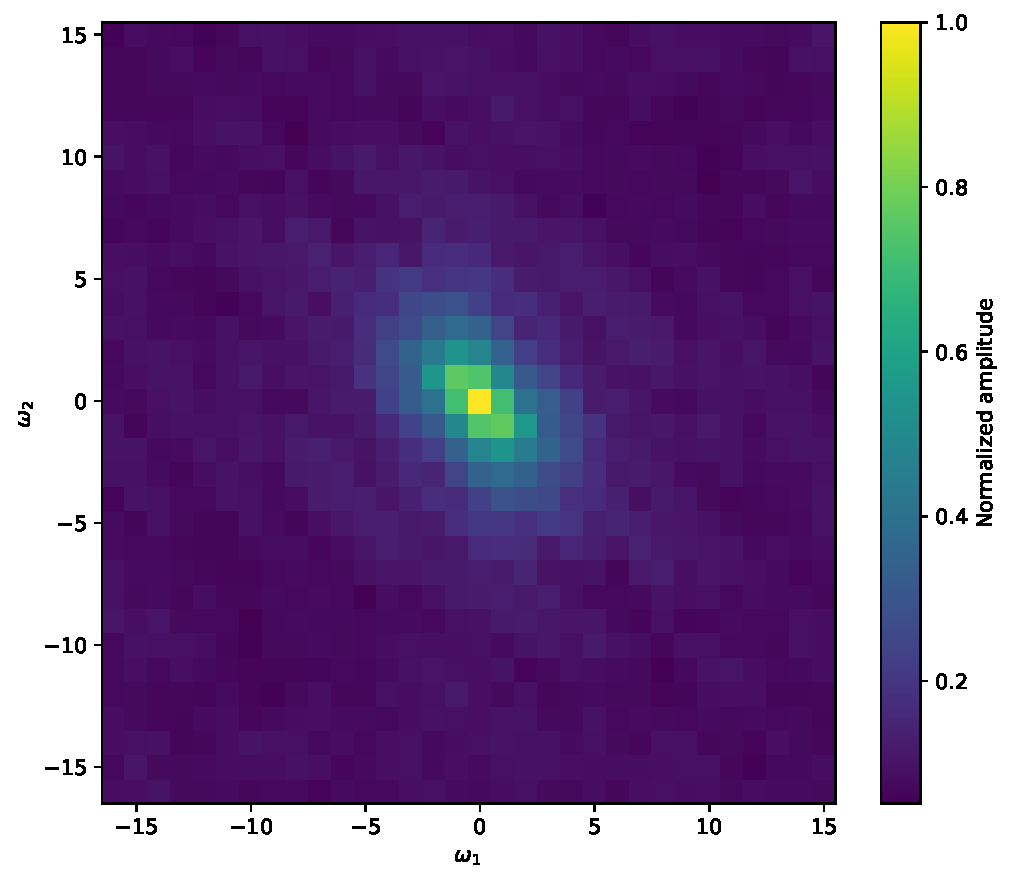
\includegraphics[width=0.6\linewidth]{pictures/plot_spectrum.pdf}
\caption{Two-dimensional projection of the normalized amplitude spectrum of the training data over the two volatility dimensions. 
The projection is obtained by summing over the strike dimension.}
\label{fig:spectrum_projection}
\end{figure}

Figure~\ref{fig:spectrum_projection} shows the projected
frequency structure of the target functions.
The multidimensional spectrum is summed over the strike dimension
and subsequently normalized, such that relative intensities
become visible.

The amplitudes are clearly concentrated in the low-frequency range.
Most of the spectral mass lies within
$|\omega_n| \leq 1$, while the intensity decreases steadily
with increasing frequency.
Frequency components with $|\omega_n| \geq 5$ are only weakly pronounced.

This structure indicates that the target functions
can predominantly be described by low frequencies.
Since the representable spectrum of a rotation-based VQC
grows with encoding depth,
a small depth is likely sufficient to capture the dominant components.
Increasing the encoding depth to cover frequencies up to approximately
$|\omega_n| \leq 4\text{--}5$ per input dimension
may further improve the approximation,
whereas beyond this range only limited additional
performance gains are to be expected.



\subsection{Model Configurations}
\label{sec:mt-model-config}

\subsubsection{Variational Quantum Circuits}

For the VQCs, encoding depths
$L \in \{1,3,4,5\}$ are considered for unary encoding,
while for ternary encoding
the encoding depths $L \in \{2,3\}$ are used.
This allows the frequency spectra computed in
Section~\ref{sec:mt-computed-spectrum} to be represented.

The size of the entire frequency spectrum for unary encoding is

\[
|\Omega| = (2L+1)^d .
\]

(cf.~Section~\ref{sec:bg-vqc-fourier}).
For ternary encoding, Equation~\ref{eq:Omega_n} yields

\[
|\Omega| = 3^{Ld}
\]

(cf.~Section~\ref{sec:bg-vqc-frequency-scaling}).

For $d=3$ input dimensions, for example,
for $L=2$ (ternary encoding) with $p_1=1$ and $p_2=3$ per dimension we obtain

\[
\Omega_n =
\{-4,-3,-2,-1,0,1,2,3,4\},
\]

such that $|\Omega_n| = 9$ and

\[
|\Omega| = |\Omega_n|^d = 9^3 = 729.
\]

For the considered encoding depths, this results in:

\begin{table}[htbp]
\centering
\begin{tabular}{c c c c}
\hline
Encoding & $L$ & Frequency range $|\omega_n|$ & $|\Omega|$ \\
\hline
Unary   & 1 & $\le 1$  & 27   \\
Unary   & 3 & $\le 3$  & 343  \\
Unary   & 4 & $\le 4$  & 729  \\
Unary   & 5 & $\le 5$  & 1331 \\
\hline
Ternary & 2 & $\le 4$  & 729  \\
Ternary & 3 & $\le 13$ & 19683 \\
\hline
\end{tabular}
\caption{Size of the achievable frequency spectrum for the considered
encoding depths with $d=3$ input dimensions.}
\label{tab:frequency-spectra}
\end{table}

To provide a sufficient number of trainable parameters for controlling
the representable Fourier coefficients,
the number of ladder sub-blocks $B$ is chosen depending on $L$ as

\[
(L,B) \in \{(1,10), (3,10), (4,17), (5,25)\}
\]

for unary encoding and

\[
(L,B) \in \{(2,20), (3,30)\}
\]

for ternary encoding.

\subsubsection{Classical Neural Networks}

For the Culkin architecture, four hidden layers
with $u=100$ neurons each and a dropout rate
of $p=0.25$ are used, corresponding to the
original configuration in the reference paper.

For the Ferguson architecture, several
variants are considered:
\begin{itemize}
    \item a configuration with $u=100$ neurons
    per hidden layer without dropout,
    analogous to the original work,
    \item as well as reduced variants with
    $u \in \{5,9,14\}$ neurons per hidden layer,
    whose number of parameters is adjusted
    to match those of the QML models.
\end{itemize}

\subsubsection{Comparison of Model Complexity}

To ensure a fair comparison between
classical neural networks and the VQC,
models with a comparable number of trainable
parameters are explicitly contrasted.
In this way, differences in predictive performance
can be attributed less to differing model capacity
and more to structural properties of the architectures.

The total number of trainable parameters
of the considered model configurations
is shown in Table~\ref{tab:model-parameters}.

\begin{table}[htbp]
\centering
\begin{tabular}{l c c}
\hline
Model & Parameters & $F_{\text{eff}}$ \\
\hline
QML (Unary, $L=1$, $B=10$) & 180 & $126$ \\
QML (Unary, $L=3$, $B=10$) & 360 & $252$ \\
QML (Unary, $L=4$, $B=17$) & 765 & $315$ \\
QML (Unary, $L=5$, $B=25$) & 1350 & $378$ \\
QML (Ternary, $L=2$, $B=20$) & 540 & $189$ \\
QML (Ternary, $L=3$, $B=30$) & 1080 & $252$ \\
\hline
Ferguson ($u = 5$) & 176 & -- \\
Ferguson ($u = 9$) & 496 & -- \\
Ferguson ($u = 14$) & 1121 & -- \\
Ferguson ($u = 100$) & 51001 & -- \\
Culkin ($u = 100$, $drop=0.25$) & 30801 & -- \\
\hline
\end{tabular}
\caption{Number of trainable parameters and maximum number of effectively controllable Fourier coefficients of the considered models.}
\label{tab:model-parameters}
\end{table}

\subsection{Baseline Scenario}
\label{sec:mt-baseline}

As a reference point for the subsequent experiments,
a baseline scenario is first considered.

In this setting, the full training dataset resulting
from the random train-test split
(cf.~Section~\ref{sec:mt-data-split})
is used. No artificial reduction
of the training data is applied.

\subsection{Reduced Training Data}
\label{sec:mt-low-data}

To investigate the generalization capability
of the models under limited data availability,
the size of the training set is reduced.

For this purpose, a random subset of the original
training dataset with
$N_{\text{train}} \in \{\;25,\;50,\;100,\;250,\;500,\;1000\}$
observations is drawn.
The test dataset remains unchanged,
ensuring comparability of the results.

\subsection{Noise Robustness}
\label{sec:mt-noise}

To examine robustness to noisy training data,
artificial noise is added to the training targets.

The noise term follows the approach proposed in
\cite{mitarai2018quantum}.
Gaussian noise of the form

\begin{equation}
    \varepsilon = \alpha \cdot \mathcal{N}(0,1)
\end{equation}

is used, where $\alpha$ denotes a scaling parameter
controlling the noise intensity.

To scale the noise relative to the magnitude
of the target values, the noise term is applied
multiplicatively to the training targets:

\begin{equation}
    \widetilde{Y}_{\text{train}} = Y_{\text{train}} \,(1 + \varepsilon).
\end{equation}

The test targets $Y_{\text{test}}$ remain unchanged
in all experiments.

The following values are considered:

\[
\alpha \in \{0, 0.05, 0.1, 0.25, 0.5\}.
\]

\subsection{Reproducibility and Random Initialization}
\label{sec:mt-seeds}

To assess the stability of the results with respect
to random influences, all experiments are repeated
over 30 different random initializations (seeds).

The respective seed affects

\begin{itemize}
    \item the random train-test split,
    \item the random selection of reduced training subsets,
    \item the realization of artificial noise,
    \item as well as the initialization of the model parameters.
\end{itemize}

The results are aggregated across all seeds.
The quantum models are fully reproducible given a fixed seed,
whereas classical neural networks may exhibit minor deviations
due to non-deterministic hardware operations and GPU-based
parallel reductions \cite{tensorflow_determinism}.

\section{Implementation Details}
\label{sec:mt-implementation-details}

The quantum machine learning models are implemented using the
\texttt{PennyLane} library \cite{bergholm2018pennylane}.
For efficient circuit evaluation, the JAX interface \cite{bradbury2018jax}
is employed.
The classical neural networks are implemented using
\texttt{TensorFlow/Keras} \cite{abadi2015tensorflow}.
For all models, fixed random seeds are used
to ensure training runs that are as reproducible as possible.
    \chapter{Results}
\label{sec:results}

\section{Baseline Performance}
\label{sec:results-baseline}

\begin{figure}[htbp]
\centering
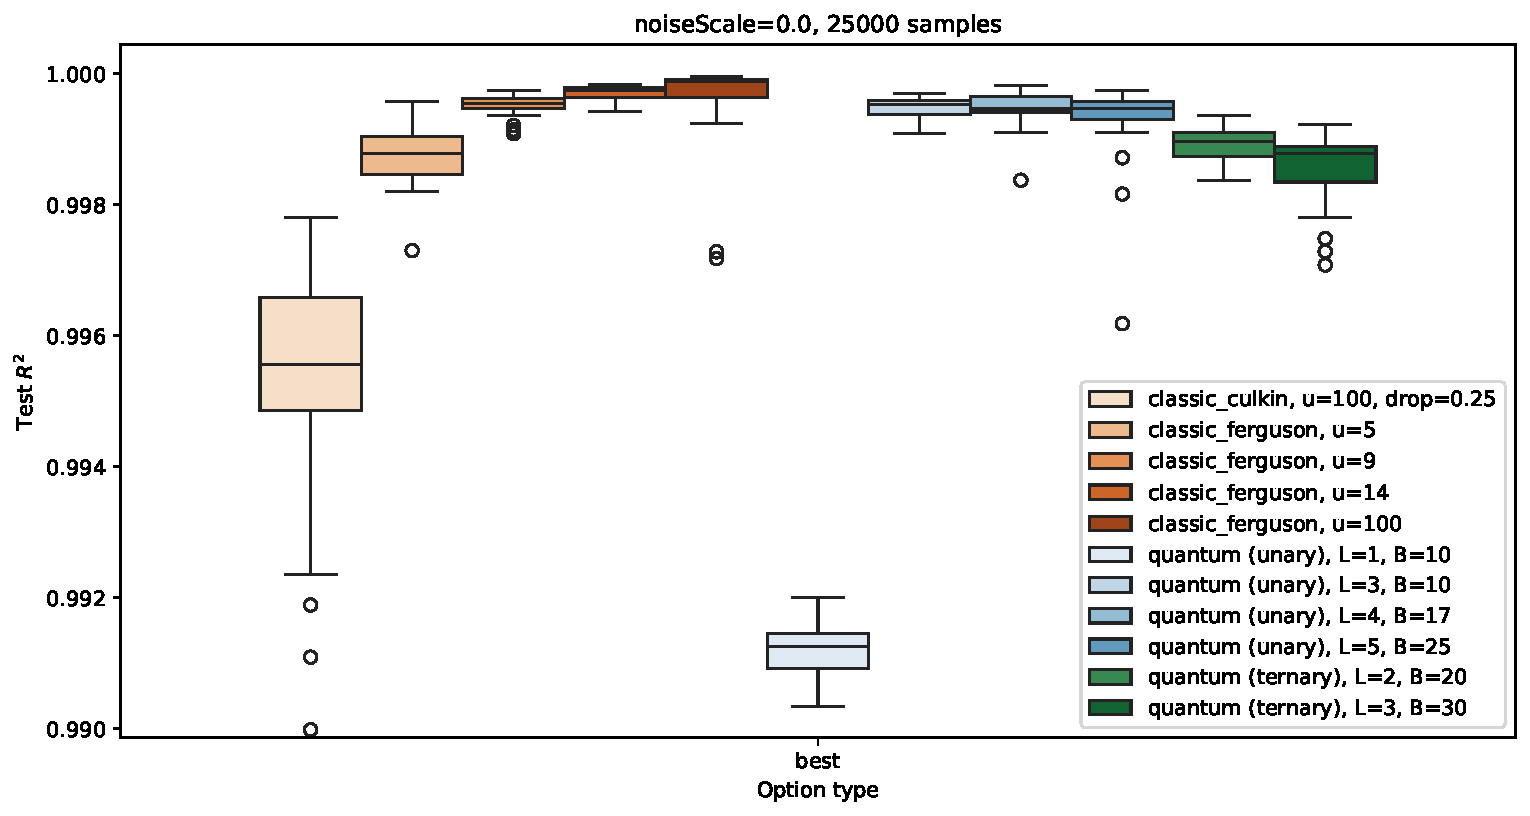
\includegraphics[width=\linewidth]{pictures/boxplot_optiontypes_nS0_nsp25k_best.pdf}
\caption{
Distribution of test-$R^2$ values across 30 seeds for Best-of basket options
in the baseline scenario (full training dataset, no artificial noise).
}
\label{fig:baseline_best}
\end{figure}

Figure~\ref{fig:baseline_best} shows the results in the baseline scenario
for Best-of options. All models achieve very high test-$R^2$ values,
indicating that the underlying pricing structure of the options can be
well approximated by the considered model architectures.

For the classical Ferguson models, a clear relationship between model
size and performance can be observed. The median test-$R^2$ increases
from $0.9988$ ($u=5$) to $0.9995$ ($u=9$), $0.9997$ ($u=14$), and
finally $0.9999$ for the largest model ($u=100$).

Despite a comparable model size, the Culkin model achieves lower
accuracy (median $R^2 = 0.9956$),
which is likely due to the use of dropout ($p=0.25$), which is not
necessary in the noise-free baseline scenario.

For the quantum models, a larger model size does not necessarily lead
to better performance. While the performance improves substantially
from the smallest model ($L=1$, median $R^2 = 0.9912$) to larger
models, only minor differences are observed afterwards. The unary
encoding models with $L=3$, $L=4$, and $L=5$ reach nearly identical
median values of approximately $0.9995$.

When comparing the encoding strategies, unary models tend to perform
slightly better than ternary models. For example, the unary model
($L=4$, $B=17$) achieves a median test-$R^2$ of $0.99946$, whereas
the ternary model with a comparable frequency spectrum ($L=2$,
$B=20$) achieves a median of $0.99897$.

For this reason, ternary models are not considered further in the
following experiments. In addition, one of the classical Ferguson
models is omitted in the subsequent experiments for improved
readability.

\begin{figure}[htbp]
\centering
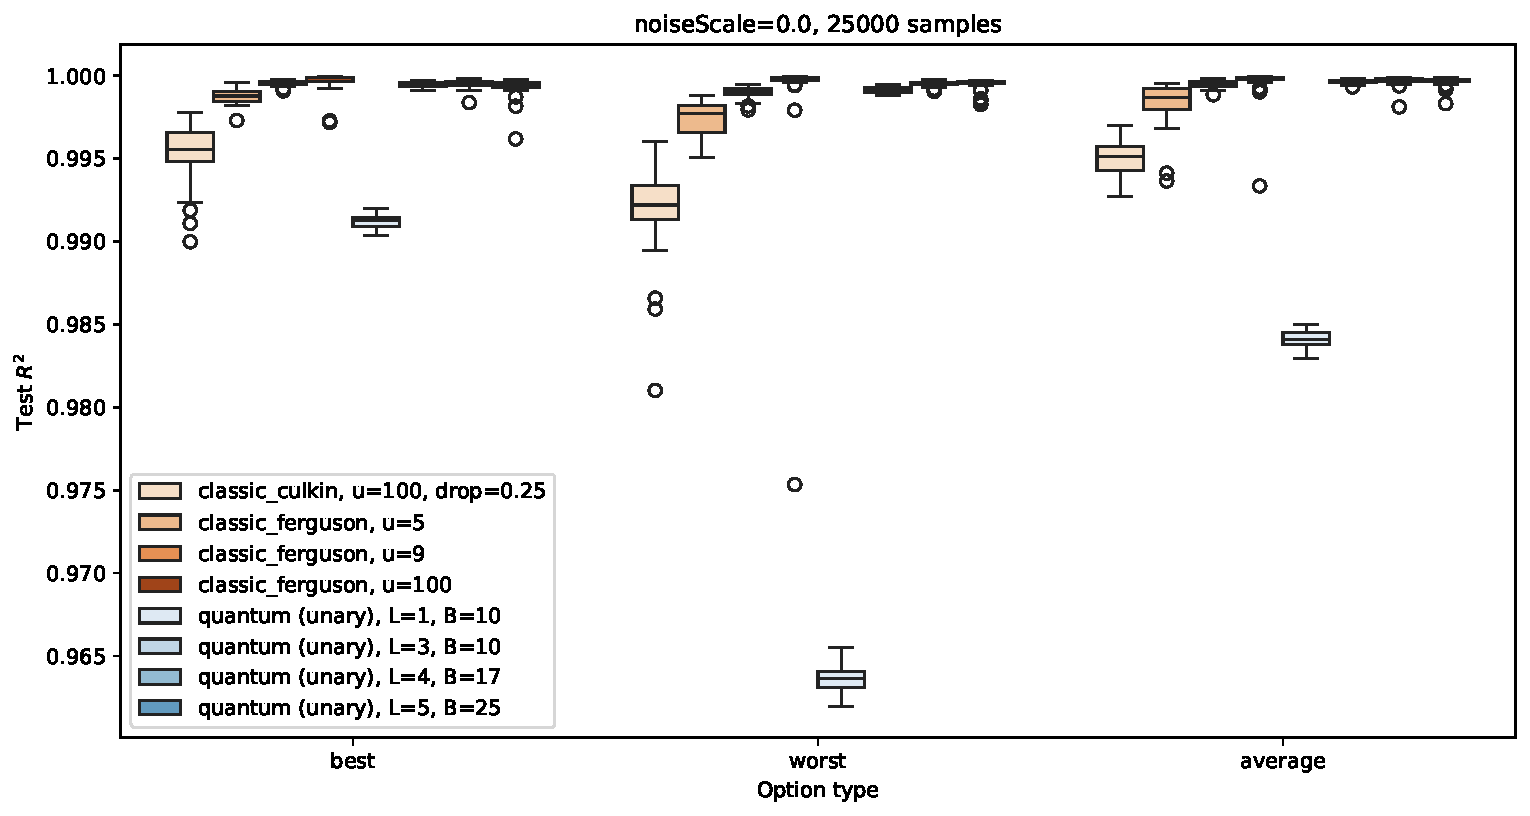
\includegraphics[width=\linewidth]{pictures/boxplot_optiontypes_nS0_nsp25k.pdf}
\caption{
Distribution of test-$R^2$ values across 30 seeds for Worst-of,
Best-of, and Average basket options in the baseline scenario
(full training dataset, no artificial noise).
}
\label{fig:baseline}
\end{figure}

Figure~\ref{fig:baseline} shows the distribution of test-$R^2$ values
for Best-of, Worst-of, and Average basket options.

For Average basket options, the results are very similar to those of
Best-of options, with median values typically exceeding $0.9995$.
For example, the Ferguson model with $u=9$ achieves a median test-$R^2$
of $0.99946$, while the largest model ($u=100$) reaches $0.99983$.
The larger quantum models also achieve high values, such as
$0.99965$ ($L=3$) and $0.99972$ ($L=4$).

The Worst-of payoff, however, represents the most challenging
approximation task. Here, the test-$R^2$ values are slightly lower
overall, particularly for the smallest quantum model ($L=1$,
median $R^2 = 0.9637$). With increasing model capacity, however,
performance improves significantly. The unary models with $L=3$,
$L=4$, and $L=5$ reach median values between approximately
$0.99906$ and $0.99958$. A similar trend can also be observed for
the classical models, where the median increases from $0.99907$
($u=9$) to $0.99986$ ($u=100$).

The slightly lower performance for the Worst-of payoff may be due to
the fact that it is not only bounded below by $0$, but also bounded
above by the value of the respective other asset. This additional
structure may complicate the approximation and lead to slightly
lower test-$R^2$ values.

For additional qualitative insights,
Figure~\ref{fig:qualitative-baseline} shows the relationship between
target values and model predictions for a representative seed in the
Worst-of scenario.

\begin{figure}[htbp]
\centering
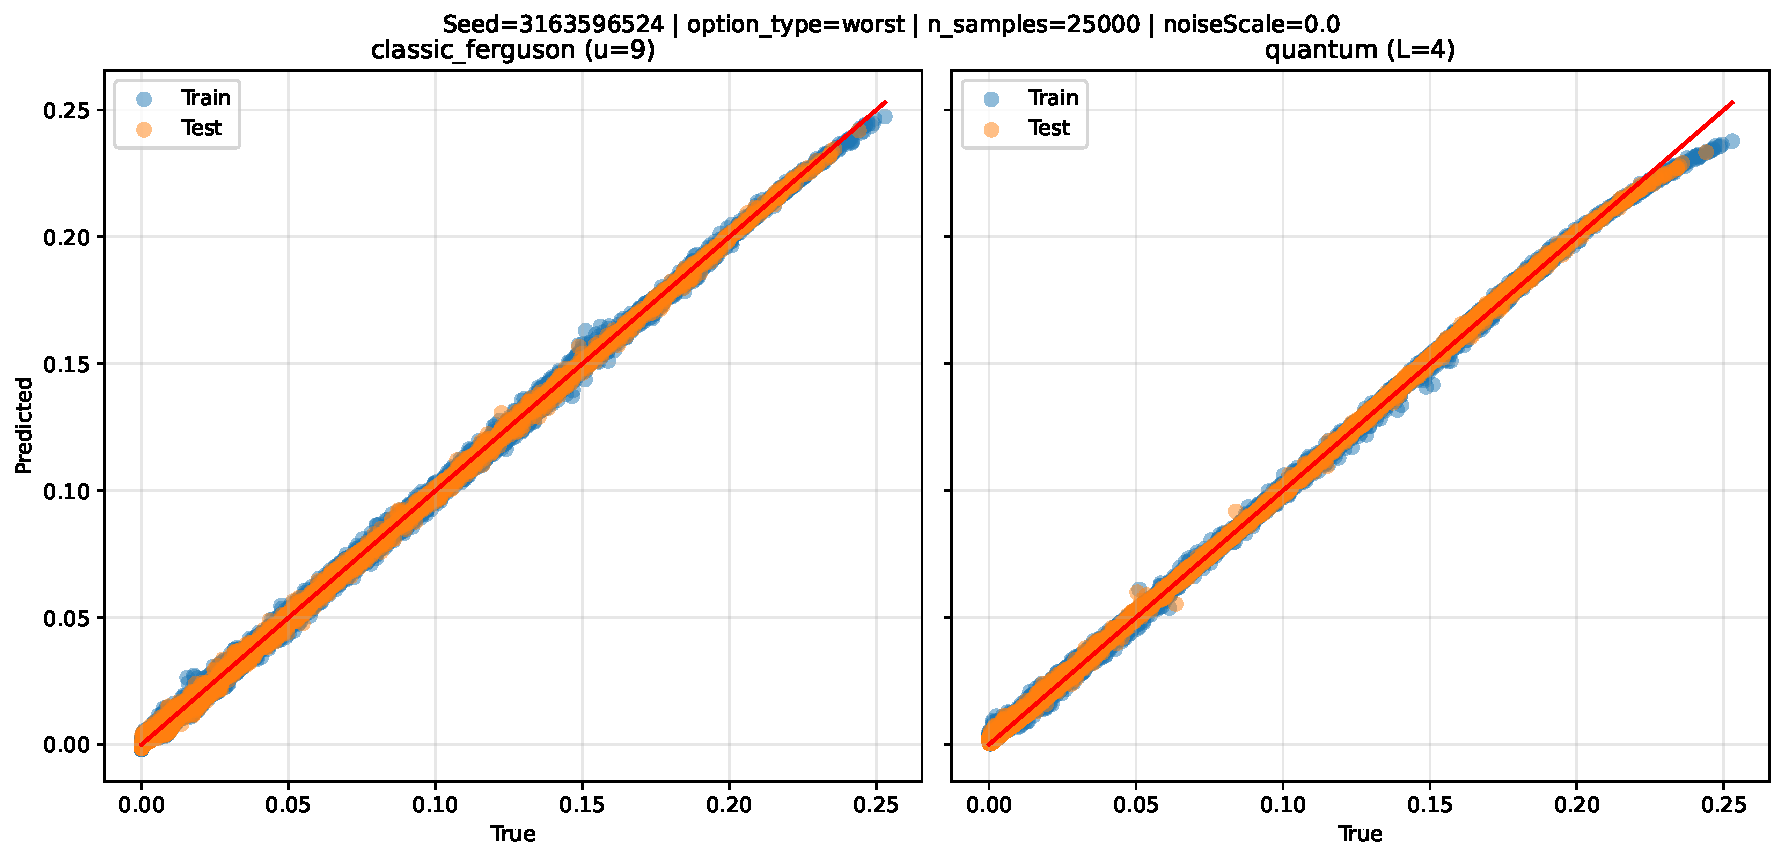
\includegraphics[width=\linewidth]{pictures/scatter_baseline.pdf}
\caption{
Predictions versus target values for a representative seed in the
baseline scenario (Worst-of, $N=25000$, $\alpha=0$). Left: Ferguson
($u=9$), right: VQC ($L=4$). The red diagonal indicates perfect
prediction.
}
\label{fig:qualitative-baseline}
\end{figure}

Both models show a strong concentration along the 45° diagonal,
which visually confirms the high test-$R^2$ values. No systematic
differences between training and test data are observable.

However, in the right panel it can be seen that the VQC tends to
systematically underestimate larger target values ($\hat{y} < y$).
The deviations increase with increasing target values, and the
point cloud shows a slightly curved structure relative to the
diagonal in the upper value range.

For further analysis, Figure~\ref{fig:error-analysis} shows the
signed error
\(
e = y - \hat{y}
\)
on the test data.

\begin{figure}[htbp]
\centering
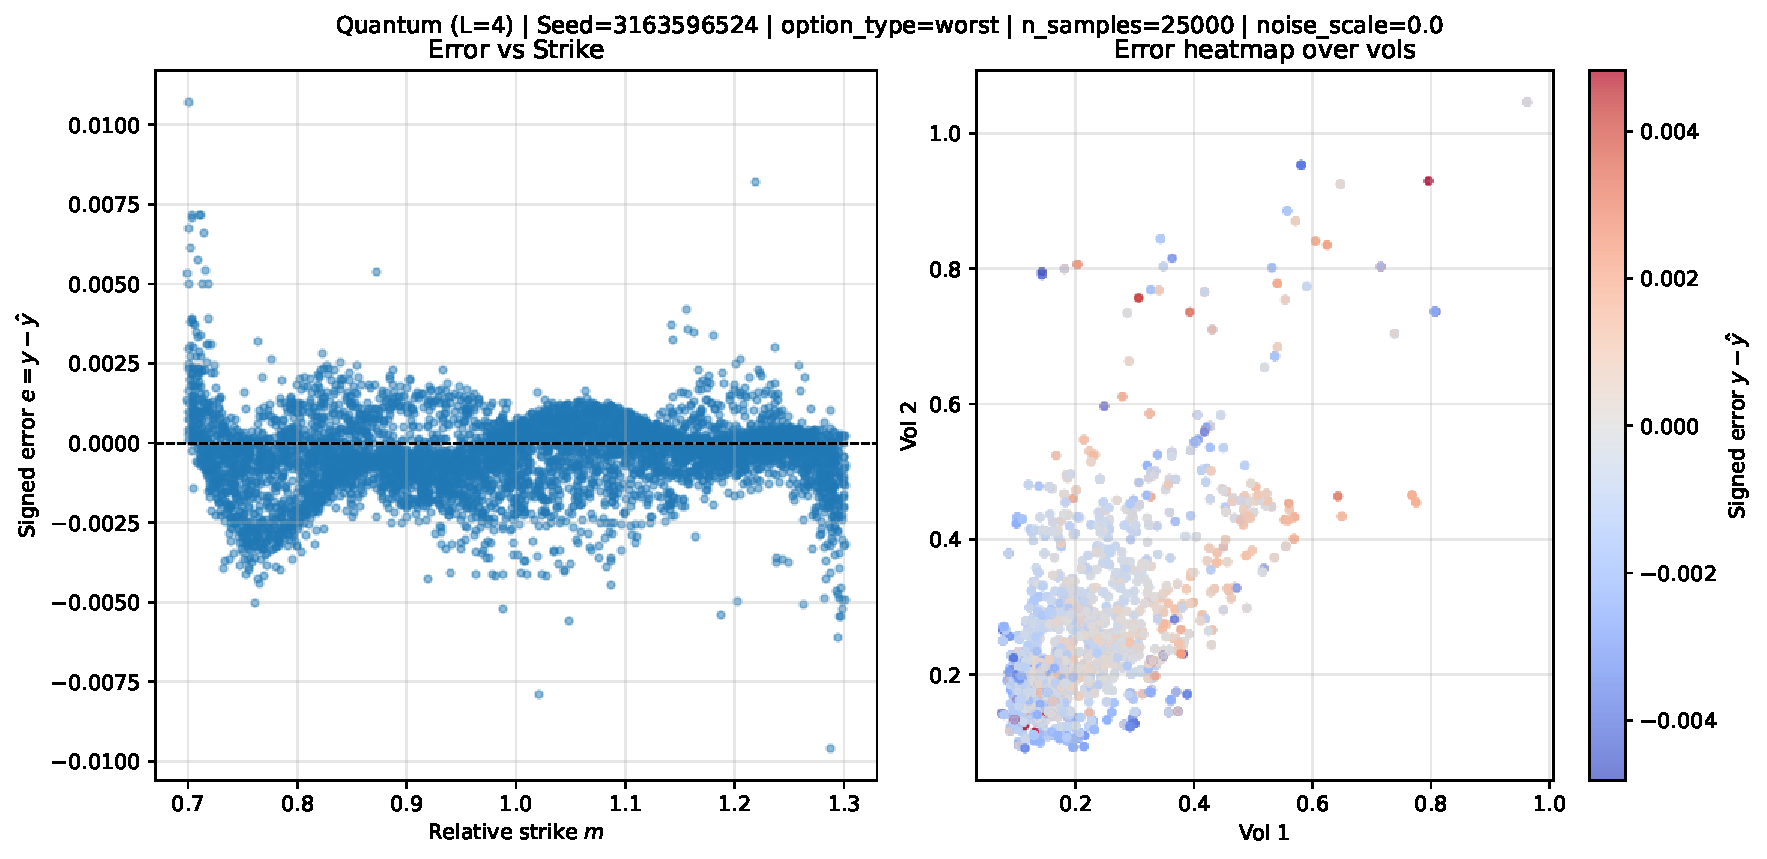
\includegraphics[width=\linewidth]{pictures/error_analysis_baseline.pdf}
\caption{
Error analysis on the test data for the same seed in the baseline
scenario. Left: error as a function of relative strike $m$. Right:
color-coded error across the two volatility dimensions.
}
\label{fig:error-analysis}
\end{figure}

Stronger positive errors occur particularly for low relative strikes
($m \approx 0.7$), corresponding to a systematic underestimation of
high option prices in this moneyness region. Since lower strikes lead
to higher option prices, this region corresponds to the upper range
of target values, which is consistent with the previously observed
underestimation of high prices.

In the projection onto the two volatility dimensions, however,
no clear spatial pattern can be identified. The errors therefore
appear to be primarily related to the strike level or the function
value itself, while no dominant relationship with specific volatility
combinations can be observed.

\section{Impact of Training Dataset Size}
\label{sec:results-samples}

\begin{figure}[htbp]
\centering
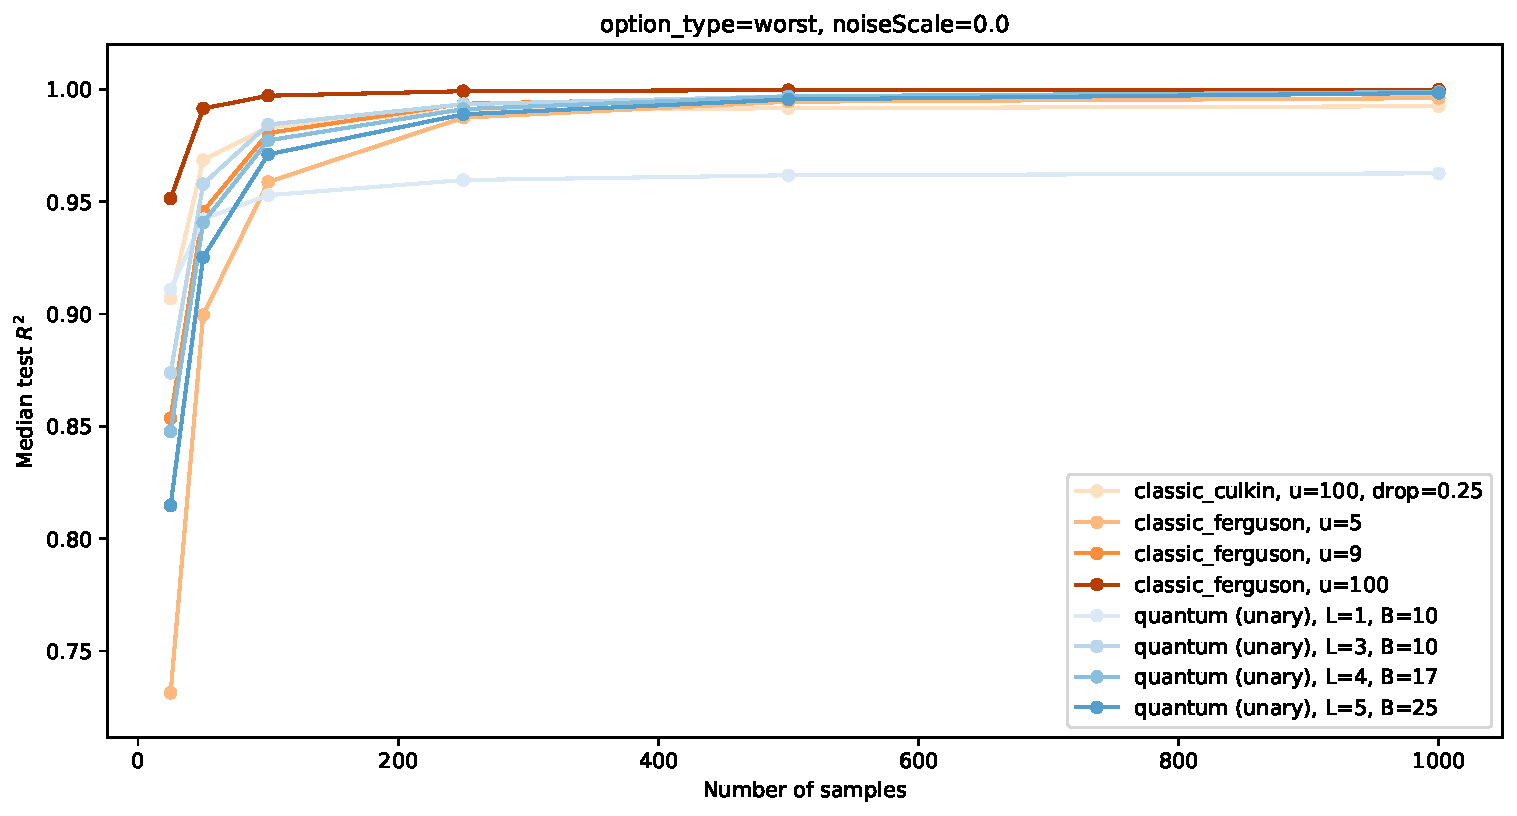
\includegraphics[width=\linewidth]{pictures/lineplot_samples0-1k_worst_nS0.pdf}
\caption{
Median test-$R^2$ as a function of the number of training observations
for the Worst-of payoff.
}
\label{fig:low_samples}
\end{figure}

Figure~\ref{fig:low_samples} shows the median test-$R^2$ for different
training dataset sizes.

For very small datasets ($N=25$), clear differences between the models
can be observed. For the classical Ferguson models, performance
increases with model size. The median $R^2$ rises from approximately
$0.73$ ($u=5$) to $0.85$ ($u=9$) and about $0.95$ ($u=100$).
The Culkin model also achieves solid results with about $0.91$,
thereby outperforming the smaller Ferguson variants.

For the quantum models, a different pattern emerges. Here, simpler
architectures appear to be more robust. The model with $L=1$ reaches
a median $R^2$ of approximately $0.91$ at $N=25$, whereas deeper
circuits perform worse ($L=3$: $\approx 0.87$, $L=4$: $\approx 0.85$,
$L=5$: $\approx 0.81$).

As the training dataset increases, the performance of all models
improves substantially. Already at $N=50$, several models achieve
$R^2$ values above $0.94$, and at $N=100$ most models exceed $0.97$.
In particular, the larger Ferguson models quickly achieve very high
accuracy; the model with $u=100$ reaches a median $R^2$ of about
$0.997$ already at $N=100$.

The VQC models also benefit from larger datasets. While shallower
architectures are more stable for small datasets, the deeper models
approach the performance of the classical networks as the amount
of training data increases. From approximately $N=250$ onwards,
the variants with $L=3$, $L=4$, and $L=5$ already reach $R^2$
values above $0.99$.

However, the simplest VQC model ($L=1$) scales more weakly.
Its median $R^2$ increases only from approximately $0.91$ at
$N=25$ to around $0.96$ at $N=1000$.

\section{Impact of Noise}
\label{sec:results-noise}

\begin{figure}[htbp]
\centering
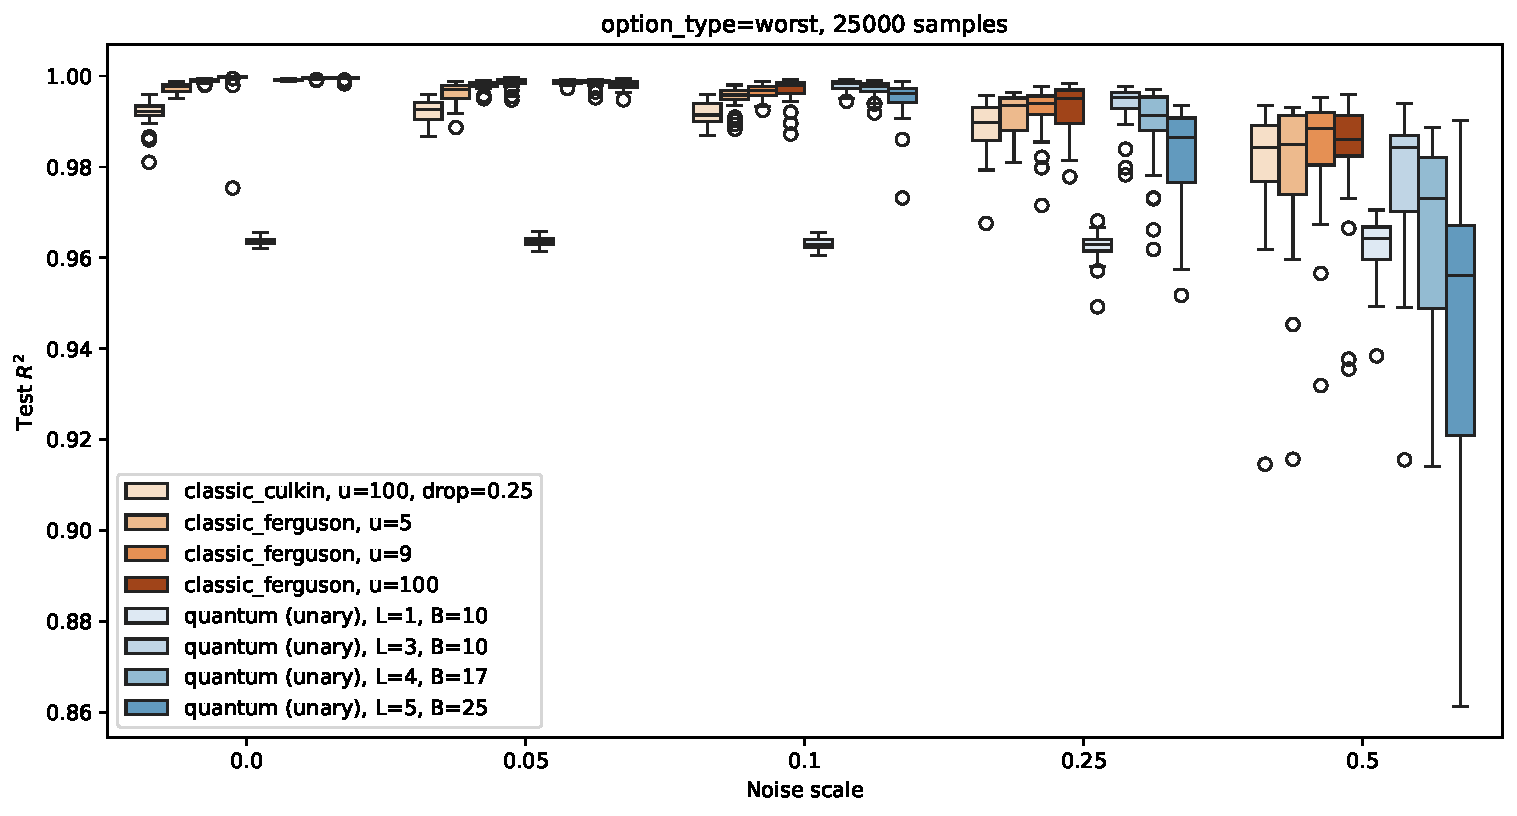
\includegraphics[width=\linewidth]{pictures/boxplot_noise_worst_25k.pdf}
\caption{
Distribution of test-$R^2$ values across 30 random initializations
for different noise intensities $\alpha$ for the Worst-of payoff
($N=25000$ training observations).
}
\label{fig:noise}
\end{figure}

Figure~\ref{fig:noise} shows the test-$R^2$ as a function of the
noise parameter $\alpha$ for the full training dataset.

At low noise intensities ($\alpha \le 0.1$), the performance of all
models remains close to the level of the baseline scenario. More
pronounced performance losses appear only at higher noise levels
($\alpha = 0.25$ and $0.5$).

The classical neural networks still achieve median values between
approximately $0.986$ and $0.988$ even at $\alpha = 0.5$. Larger
Ferguson architectures tend to show stronger absolute performance
declines. For example, the median for the largest model ($u=100$)
decreases from $0.99986$ in the baseline scenario to about $0.986$.

The Culkin model with dropout proves to be relatively robust. The
median test-$R^2$ decreases only from approximately $0.992$ to about
$0.984$, which can plausibly be attributed to the regularizing effect
of dropout.

For the VQC models, the sensitivity to noise strongly depends on the
circuit depth. The shallowest model ($L=1$) remains relatively stable
across all noise levels ($R^2 \approx 0.96$), although it already
achieves lower accuracy in the baseline scenario.

As the depth increases, the sensitivity to noise also increases.
While the model with $L=3$ still achieves about $0.984$ at
$\alpha = 0.5$, the median values for $L=4$ and $L=5$ drop to
approximately $0.973$ and $0.956$, respectively.

Overall, the results indicate that larger model capacity offers
advantages in the noise-free case but leads to stronger performance
degradation under increasing noise. Shallower models appear more
robust, although they are limited in their maximum approximation
capability.

\section{Combined Impact of Noise and Sample Size}
\label{sec:results-noise-samples}

\begin{figure}[htbp]
\centering
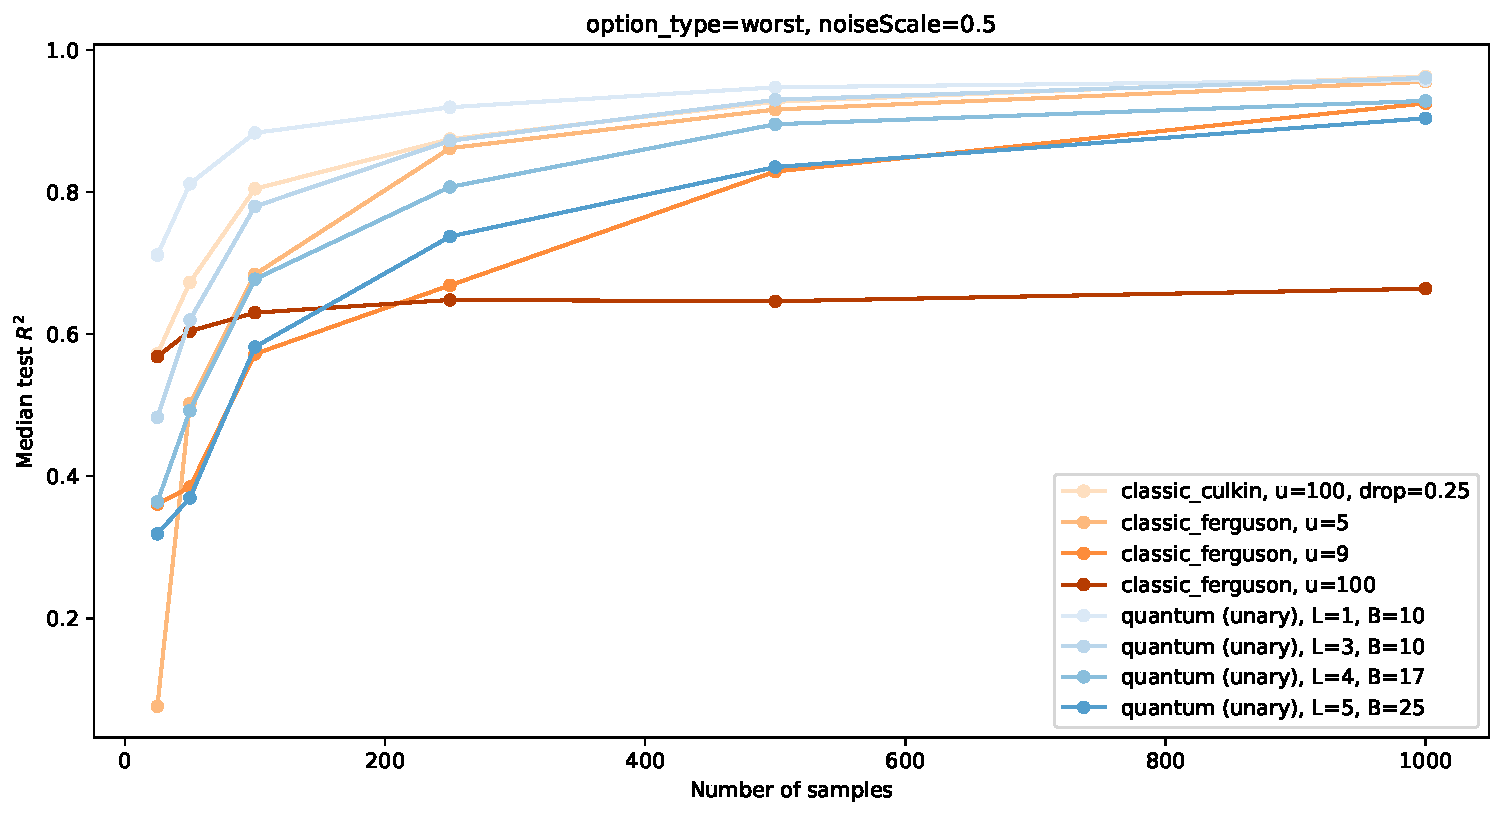
\includegraphics[width=\linewidth]{pictures/lineplot_samples0-1k_worst_nS05.pdf}
\caption{
Median test-$R^2$ as a function of training dataset size for the
Worst-of payoff under strong noise ($\alpha = 0.5$).
}
\label{fig:noise_samples}
\end{figure}

Figure~\ref{fig:noise_samples} shows the median test performance
for the combined scenario of strong training noise ($\alpha = 0.5$)
and varying training dataset size.

For very small datasets ($N=25$), the model architectures differ
substantially. The simplest VQC model ($L=1$) achieves the best
results with a median $R^2$ of about $0.71$, whereas deeper
variants perform considerably worse ($L=5$: $\approx 0.32$).

As the training dataset size increases, the deeper VQC models
improve substantially. At $N=1000$, the model with $L=1$ reaches
approximately $0.96$, while $L=3$ performs slightly better with
$R^2 \approx 0.961$. The models with $L=4$ and $L=5$ also benefit
strongly from larger datasets and reach approximately $0.93$
and $0.90$, respectively.

For the Ferguson architectures, a different pattern emerges.
At $N=25$, the largest model ($u=100$) achieves the best result
within this model family with about $0.57$, but still performs
considerably worse than the VQC model with $L=1$. The smallest
Ferguson model ($u=5$) performs particularly poorly with
$R^2 \approx 0.08$.

With increasing training dataset size, especially the smaller
Ferguson models improve substantially. The model with $u=5$
reaches a median $R^2$ of approximately $0.96$ at $N=1000$
and thus becomes one of the best-performing classical
architectures. In contrast, the largest Ferguson model
($u=100$) shows only limited improvement (from about $0.57$
to about $0.66$).

The Culkin model also benefits strongly from larger datasets.
Its median $R^2$ increases from about $0.57$ ($N=25$) to
approximately $0.96$ ($N=1000$), making it one of the best
performing classical models for larger datasets.

Overall, a clear trade-off between model capacity and data
availability can be observed. Simpler models are more robust
for very small datasets, whereas more complex architectures
reach their full potential only when sufficient training data
are available.


\section{Temporally Ordered Train-Test Split}
\label{sec:results-time-split}

\begin{figure}[htbp]
\centering
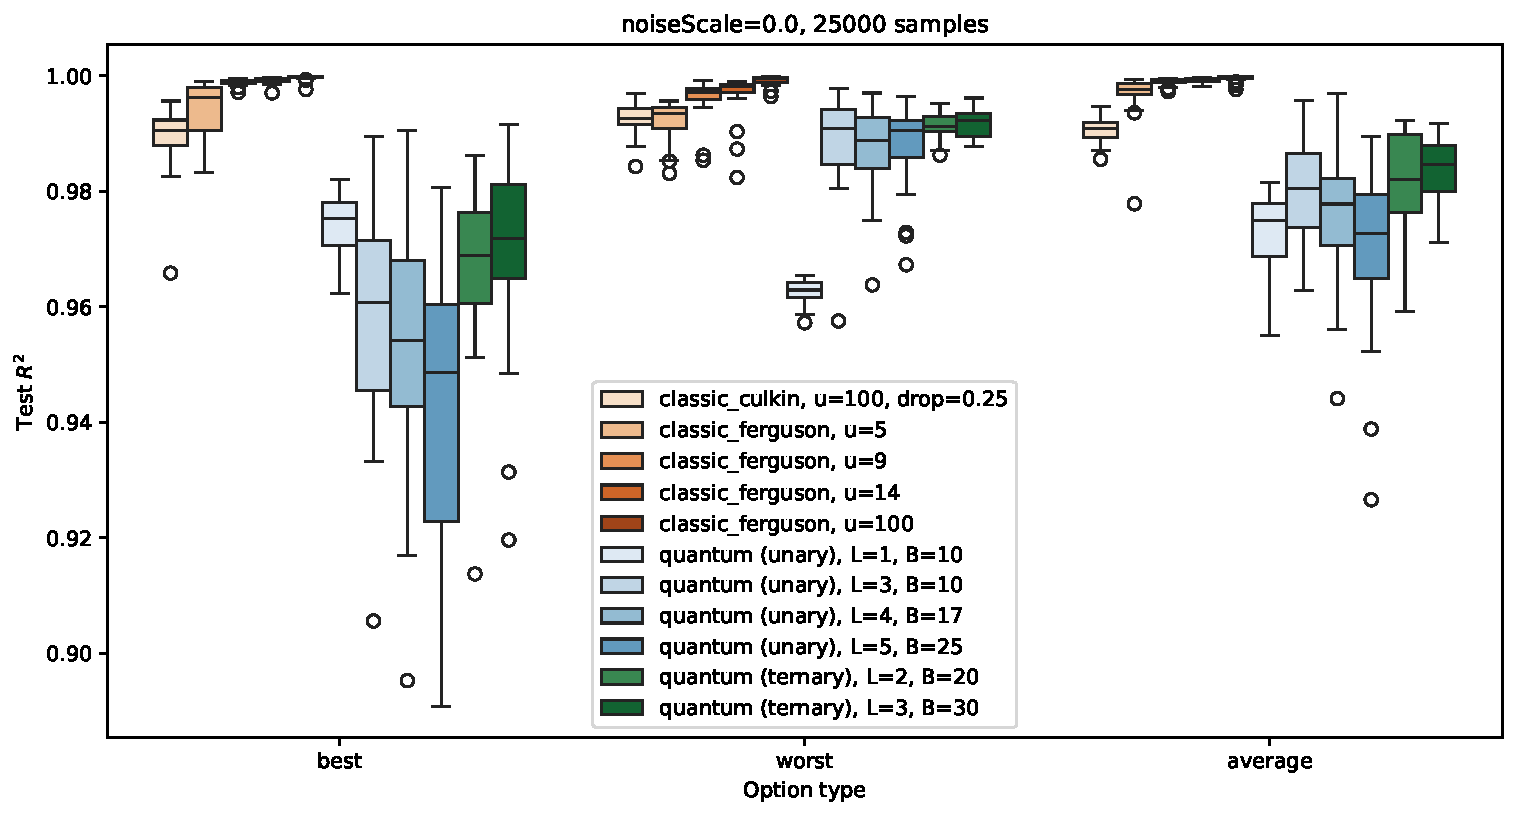
\includegraphics[width=\linewidth]{pictures/boxplot_optiontypes_nS0_nsp25k_time.pdf}
\caption{
Distribution of test-$R^2$ values across 30 seeds for Worst-of,
Best-of, and Average basket options in the baseline scenario with
a temporally ordered train–test split ($N=25000$, $\alpha=0$).
}
\label{fig:time_split}
\end{figure}

Figure~\ref{fig:time_split} shows the test-$R^2$ values for a temporally
ordered train–test split, in which only earlier observations are used
for training and later observations for testing.

The classical models largely retain their high predictive performance.
In particular, the larger Ferguson architectures continue to achieve
very high median values. For Average basket options, the median
test-$R^2$ increases from $0.9977$ ($u=5$) to $0.9991$ ($u=9$),
$0.9992$ ($u=14$), and $0.9997$ for the largest model ($u=100$).
The Culkin model performs slightly worse but still achieves high
values ($R^2 \approx 0.991$ for Average and $0.993$ for Worst-of).

In contrast, the VQC models show a noticeably stronger deterioration
compared to the random train–test split, particularly for the
Best-of payoff. Here, the median $R^2$ decreases with increasing
circuit depth from about $0.975$ ($L=1$) to $0.961$ ($L=3$),
$0.954$ ($L=4$), and $0.949$ ($L=5$).

Models with ternary encoding perform slightly better in this
scenario than the larger unary variants. For Best-of options,
they reach median values of approximately $0.969$ ($L=2$) and
$0.972$ ($L=3$).

For Worst-of options, the differences between the quantum models
are considerably smaller. The median values of the unary models
with $L=3$–$5$ lie between approximately $0.989$ and $0.991$,
while the ternary models reach similar values between
approximately $0.991$ and $0.992$.

Since the Best-of payoff is approximated significantly worse by
the quantum models under the temporally ordered split, this case
is examined in more detail. Figure~\ref{fig:error-analysis-timesplit-bestof}
shows the error structure in the Best-of scenario.

\begin{figure}[htbp]
\centering
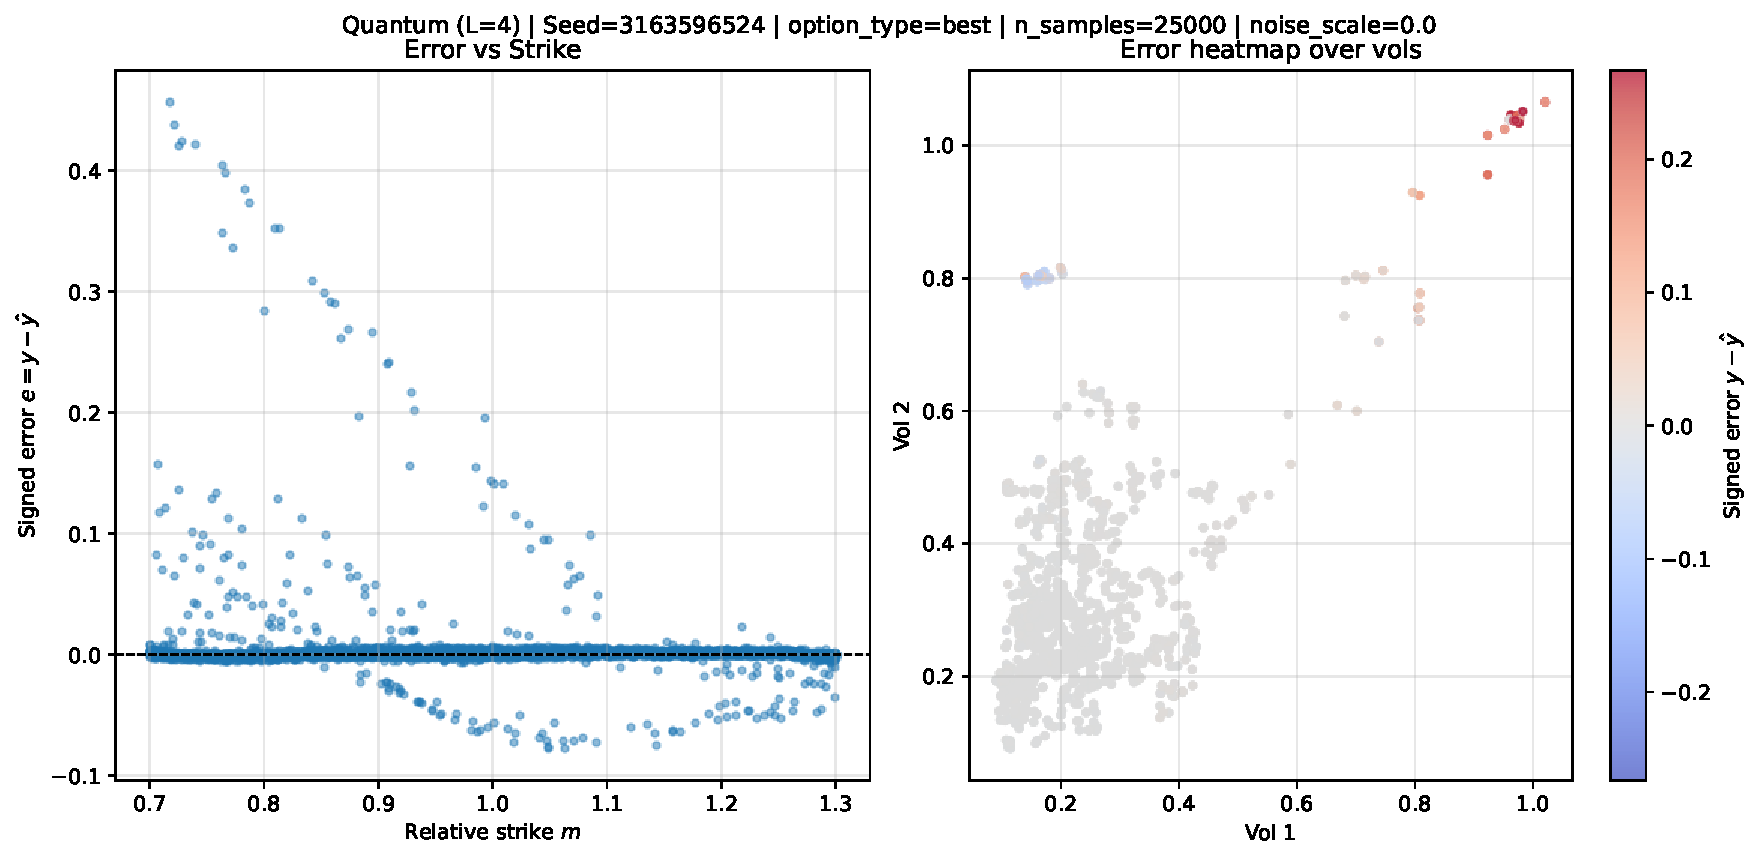
\includegraphics[width=\linewidth]{pictures/error_analysis_timesplit.pdf}
\caption{
Error analysis under the temporally ordered split (Best-of).
Left: error as a function of the relative strike.
Right: projection onto the volatility dimensions.
}
\label{fig:error-analysis-timesplit-bestof}
\end{figure}

Positive errors occur particularly for low strikes, corresponding
to a systematic underestimation of high option prices. In addition,
in contrast to the random train–test split, a clear concentration
of larger errors can be observed at simultaneously high volatility
levels.

Since a temporally ordered split is used, Figure~\ref{fig:vol-timesplit}
illustrates the temporal evolution of the rolling volatilities
together with the locations of the largest prediction errors.

\begin{figure}[htbp]
\centering
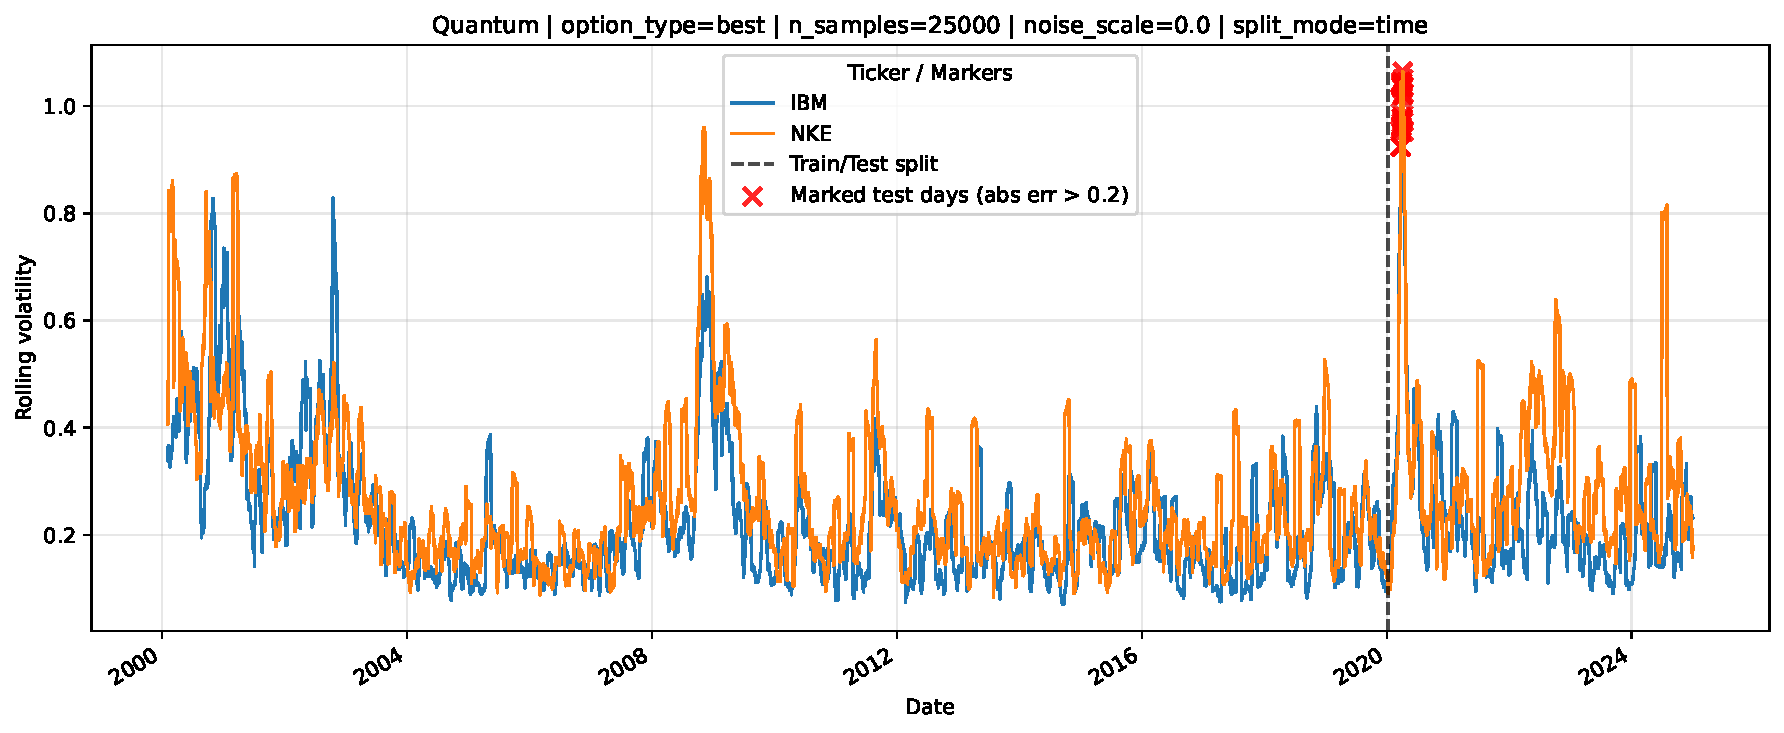
\includegraphics[width=\linewidth]{pictures/vol_timesplit_marked.pdf}
\caption{
Rolling volatilities with marked test days exhibiting large errors.
The dashed line indicates the boundary between the training and
test periods.
}
\label{fig:vol-timesplit}
\end{figure}

The highest volatility levels occur exclusively during the test
period. Large prediction errors concentrate in these phases,
while comparable volatility levels are not observed during the
training period. This indicates a distribution shift between
the training and test periods in the volatility features.
    \chapter{Discussion}

\section{Model Capacity and Frequency Structure}

In the baseline scenario, almost all models achieve very high predictive
performance. The performance increase of the VQC when moving from
$L=1$ to $L=3$ (unary) or $L=2$ (ternary), followed by only marginal
improvements thereafter, can be explained by the previously analyzed
frequency structure. The target functions are dominated by
low-frequency components, so that even small encoding depths capture
most of the relevant structure. Increasing the depth further expands
the representable frequency spectrum, but provides only limited
additional benefit since high-frequency components are only weakly
present in the target functions.

The lower performance of the ternary models can also be explained by
their smaller number of effective parameters. Since ternary encoding
can represent a comparable frequency spectrum with fewer layers, the
number of effectively usable parameters is more strongly limited by
the achievable DLA.

Systematic differences can also be observed between the different
payoff structures. The Worst-of payoff represents the most challenging
approximation task. In contrast to Best-of and Average payoffs, the
function is not only bounded below by zero but is additionally defined
by a minimum operator. This structure introduces stronger nonlinearities
and therefore leads to slightly lower median $R^2$ values. These
nonlinearities are particularly pronounced near the payoff boundary,
where the option value transitions from zero to positive values.
Outside this region, the pricing function often behaves approximately
linearly, since changes in the input variables affect the payoff more
proportionally.

In the Worst-of scenario, the VQC also exhibits systematic positive
errors at low relative strikes in the upper value range, corresponding
to an underestimation of high option prices. In this region, the payoff
depends strongly on the minimum of the underlying assets, so that small
changes in the inputs can lead to larger changes in the function value.

Rotation-based VQCs can be interpreted functionally as models with a
finite Fourier-like frequency spectrum. Non-smooth or kink-like
structures can therefore only be approximated, while the globally
coupled parametrization induces a certain smoothing effect. This is
consistent with the observed underestimation of high target values
(Figure~\ref{fig:error-analysis}).

\section{Impact of Model Capacity under Limited Data}

With reduced training data, a more differentiated picture emerges.
Large Ferguson architectures maintain high predictive performance even
for very small datasets, suggesting that their larger model capacity
already provides an advantage with limited data and does not lead to
pronounced overfitting effects.

The Culkin model also shows stable performance for small datasets,
which is likely related to the regularizing effect of the applied
dropout.

In contrast, the VQC models exhibit an opposite pattern. The shallow
configuration ($L=1$) is the most robust for very small datasets,
whereas deeper variants show noticeable performance degradation. This
can be explained by the strongly expanded frequency representation at
larger encoding depths. If the training data are insufficient to
reliably determine additional degrees of freedom, unstable
approximations may occur. The shallow configuration therefore acts
like a more strongly regularized model.

As the amount of training data increases, this picture changes.
Once sufficient data are available, the deeper VQC architectures also
benefit from their larger model capacity and achieve predictive
performance comparable to classical networks.

\section{Robustness to Noise}

The experiments with artificial noise show that models with high
capacity achieve the best results in the noise-free case, but suffer
disproportionate performance losses as noise intensity increases. This
applies both to large Ferguson architectures and to VQCs with greater
encoding depth.

Nevertheless, the classical neural networks remain relatively robust
to moderate noise and still achieve high test-$R^2$ values even at
$\alpha = 0.5$.

The Culkin model with dropout shows particularly high stability,
which can plausibly be attributed to the regularizing effect of
dropout.

The shallow VQC ($L=1$) also exhibits only minor performance losses,
whereas deeper variants are considerably more sensitive to noisy
training data.

These observations can be explained by the effective model complexity.
Models with greater capacity possess more degrees of freedom and can
therefore more easily adapt to noise in the training data, whereas
simpler architectures act as stronger regularizers and thus remain
more robust.

\section{Interaction of Data Scarcity and Noise}

In the combined scenario of limited training data and strong noise,
this pattern becomes even more apparent. Models with lower capacity
achieve more stable results for very small datasets than more complex
architectures.

In particular, the shallow VQC remains one of the most robust
configurations across all considered sample sizes, whereas deeper
variants perform substantially worse when the dataset is very small.

As the amount of training data increases, however, this picture
changes considerably. Once sufficient data are available, the deeper
VQC models benefit from their greater expressive power and strongly
improve their predictive performance.

For the classical architectures, a similar but not identical effect
can be observed. While smaller Ferguson models benefit substantially
from increasing dataset size, very large models show only limited
improvement under strong noise when additional training data are
provided.


\section{Generalization under a Temporally Ordered Split}

Such a split is also closer to the real application scenario in
financial contexts, since models are typically trained on historical
data and applied to future market periods. While the classical
architectures largely retain their high predictive performance,
the VQC models show increased sensitivity, particularly in the
Best-of scenario.

The analysis shows that higher volatility levels occur during the
test period than were observed during training. The largest prediction
errors concentrate in these phases, indicating a distribution shift
(out-of-distribution) in the volatility features. In the Best-of case,
target values also appear that systematically exceed the range
observed during training.

This effect is particularly pronounced in the Best-of scenario.
Higher volatility increases the probability of extreme terminal
values of individual underlyings. Since the Best-of payoff is
determined by the maximum, this leads to more pronounced extreme
values and a steeper functional behavior than for Worst-of or
Average payoffs. Consistent with this, the performance degradation
of the VQC models is considerably smaller for Worst-of.

The deterioration is particularly visible for deeper VQC
configurations. One possible explanation is that greater encoding
depth improves interpolation within the training distribution,
but at the same time increases sensitivity to distribution shifts.
Classical ReLU-based architectures approximate functions in a
piecewise linear manner and extend learned slopes beyond the
training region, which may lead to more robust generalization in
this scenario.

\section{Limitations}

The original goal of this work was to study basket option prices
based on real observed market data, in order to represent the
correlations between the underlying assets using entanglement.
However, since hardly any freely available historical datasets
exist for actual basket option prices, the target values were
generated synthetically using Monte Carlo simulations.

Although the simulation is based on real historical time series
of the underlying assets, it represents a model-based
approximation. In particular, simplifying assumptions such as
constant correlations and simplified dynamics are made.
Consequently, the dependencies between the assets represented
through entanglement may differ from those observed in real
market prices.

The resulting target values therefore reflect the complexity of
real market prices only to a limited extent.

\section{Future Work}

A natural extension of this work is the use of more complex and
realistic datasets. In the present experiments, basket option
prices were generated using a simplified simulation model whose
frequency structure is dominated by low-frequency components.
Future work could investigate how the models behave when the
target functions exhibit more pronounced high-frequency
structures.

One possible direction is the use of real market data for basket
options, provided that suitable datasets become available.
Alternatively, more realistic simulation models could be
employed, for example incorporating time-dependent correlations,
stochastic volatility, or varying maturities.

Furthermore, it would be interesting to analyze to what extent
modeling absolute basket prices instead of relative returns
changes the functional structure of the target variable and
therefore imposes different requirements on the frequency
representation.

Another extension is the consideration of a larger number of
underlying assets. As dimensionality increases, the structural
complexity of the pricing function grows substantially. Since
the representable frequency spectrum of rotation-based VQCs
increases exponentially with the input dimension, more
pronounced differences between classical and quantum-based
models may emerge in higher-dimensional settings.

Finally, it could be investigated whether appropriate
preprocessing of the target variable improves modeling.
Since option prices are nearly linear across large regions of
the input space and stronger nonlinearities mainly occur near
the payoff boundaries, a transformation such as an arccos
mapping could help distribute the functional structure more
evenly and thereby facilitate approximation by rotation-based
VQCs.
    \chapter{Conclusion}

A central motivation of this work was the question of whether the
ability of entangled quantum states to represent non-separable
dependencies can provide advantages when modeling the correlations
between multiple underlyings on which basket options depend.
Against this background, this thesis investigated the extent to
which VQCs are suitable for approximating basket option prices.
To assess their performance, a comparison with established classical
neural network architectures was conducted.

The results show that both classical neural networks and VQC-based
models are able to approximate the underlying pricing function of
basket options with high accuracy. In the baseline scenario with a
large training dataset and without artificial noise, almost all
models achieve test-$R^2$ values close to $1$. This confirms that
data-driven approaches are generally well suited to learn complex
valuation functions in the context of option pricing.

The analysis of model capacity reveals notable differences between
classical architectures and VQC models. While classical neural
networks tend to show continuous performance improvements as the
model size increases, VQCs already achieve most of their maximum
performance at moderate circuit depth. Additional layers expand
the representable frequency spectrum, but provide only limited
benefit in the considered datasets since the target functions are
dominated by low-frequency components.

Under limited data availability, a clear trade-off between model
capacity and robustness can be observed. Simpler architectures --
both classical networks and VQCs -- produce more stable results for
small datasets, whereas more complex models reach their full
potential only when sufficient training data are available.
A similar pattern appears under noisy training data, where models
with higher capacity suffer stronger performance degradation.
This effect becomes particularly pronounced in the combined
scenario of limited data and strong noise, where simpler models,
especially shallow VQCs and smaller classical networks, show the
most robust performance.

The analysis of a temporally ordered train–test split further
reveals differences in generalization behavior. While classical
ReLU-based networks largely retain their predictive performance,
VQCs show greater sensitivity to distribution shifts in the
input features, particularly at higher volatility levels.
This suggests that the globally coupled functional structure
of rotation-based quantum models allows highly accurate
approximation within the training distribution but may lead
to less robust extrapolation.

Overall, the results demonstrate that VQC-based models can achieve
competitive approximation performance for basket option pricing.
However, no clear practical advantage over classical neural
networks can be identified in the investigated setting.
At the same time, the experiments highlight that their performance
strongly depends on the structure of the target function as well
as on data availability, data quality, and the stability of the
data distribution.
    \chapter*{Transparency and Reproducibility}
\addcontentsline{toc}{chapter}{Transparency and Reproducibility}

\section*{Reproducibility}
The full source code used in this thesis is available at:
\url{https://github.com/moritz-maier/Basket-Option-Pricing-with-Quantum-Circuits}.

\section*{Use of AI Tools}
Large Language Models, specifically ChatGPT, were used during the preparation of this thesis for translation,
language editing, text refinement, assistance with debugging code, support in generating plotting scripts,
and for generating and refining code comments.

    % \input{text/introduction-UTF8}
    %\input{text/introduction-ISO8859-1}
    % further chapters
%
% =================================================================================================
% place your appendix here
% -------------------------------------------------------------------------------------------------
%
    % \appendix
    % \input{text/appendix}
    % further appendix
%
% =================================================================================================
% comment \listoffigures and/or \listoftables if not wanted
% -------------------------------------------------------------------------------------------------
%
    \backmatter
    \listoffigures                                % list of figures (uncomment if wanted)
    \listoftables                                 % list of tables (uncomment if wanted)
    % \lstlistoflistings                            % list of listings (uncomment if wanted)
%
% =================================================================================================
% place your bibliography here
% -------------------------------------------------------------------------------------------------
%
    \begin{spacing}{0.9}                          % save some space
       % \bibliographystyle{geralpha}               % for german thesis
       \bibliographystyle{alpha}                 % for english thesis
       \bibliography{bibliography}                % the location of bib file
    \end{spacing}

\end{document}
%
% =================================================================================================
% end of document
% -------------------------------------------------------------------------------------------------
%
